\documentclass[10pt,landscape]{article}

% --- Configuración de Página y Geometría ---
\usepackage[utf8]{inputenc}
\usepackage[T1]{fontenc}
\usepackage{lmodern}
\usepackage[letterpaper,landscape,top=0.55cm,bottom=0.65cm,left=0.65cm,right=0.65cm]{geometry}
\usepackage{xcolor}
\usepackage{listings}
\definecolor{codebg}{RGB}{15, 23, 42}       % Dark Slate 900
\definecolor{codegreen}{RGB}{52, 211, 153}   % Emerald 400
\definecolor{codeblue}{RGB}{56, 189, 248}    % Sky 400
\definecolor{codeamber}{RGB}{251, 191, 36}   % Amber 400
\definecolor{codegray}{RGB}{148, 163, 184}   % Slate 400

\lstdefinestyle{solvanta_python}{
    backgroundcolor=\color{codebg},
    commentstyle=\color{codegray}\itshape,
    keywordstyle=\color{codeblue}\bfseries,
    stringstyle=\color{codegreen},
    basicstyle=\fontsize{4.6pt}{5.5pt}\ttfamily\color{white},
    breaklines=true,
    numbers=left,
    numberstyle=\tiny\color{codegray!80},
    numbersep=3pt,
    showstringspaces=false,
    tabsize=2,
    frame=none
}

% --- Paquetes Matemáticos y de Tablas ---
\usepackage{amsmath,amssymb}
\usepackage{booktabs}

\usepackage{tabularx}
\usepackage{colortbl}
\usepackage{microtype}
\newcolumntype{Y}{>{\centering\arraybackslash}X}
\newcolumntype{L}{>{\raggedright\arraybackslash}X}
\newcolumntype{R}{>{\raggedleft\arraybackslash}X}
\usepackage{array}
\usepackage{xcolor}
\usepackage{graphicx}
\graphicspath{{scratch/}{./scratch/}{./}{../scratch/}{../../scratch/}{_auxiliar_local/backup_workspace_externo_pre_reorganizacion/scratch/}}
\usepackage{tcolorbox}
\tcbuselibrary{skins,breakable}
\usepackage{fancyhdr}
\usepackage{enumitem}
\usepackage{lastpage}

% --- Paleta de Colores Corporativa Solvanta ---
\definecolor{navyblue}{RGB}{10, 37, 64}        % #0A2540 Azul corporativo Solvanta
\definecolor{accentcyan}{RGB}{0, 164, 214}     % #00A4D6 Cyan tecnológico
\definecolor{softblue}{RGB}{240, 246, 252}     % Fondo azul suave
\definecolor{emeraldgreen}{RGB}{5, 150, 105}   % #059669 Verde éxito / cumplimiento
\definecolor{darkred}{RGB}{185, 28, 28}        % #B91C1C Rojo oscuro alta visibilidad
\definecolor{amber}{RGB}{180, 83, 9}           % #B45309 Ámbar energía / calor visible
\definecolor{tableheader}{RGB}{18, 53, 91}     % Azul encabezado de tabla
\definecolor{roweven}{RGB}{255, 255, 255}      % Blanco fila par
\definecolor{rowodd}{RGB}{245, 249, 253}       % Gris azulado suave fila impar
\definecolor{badgegreen}{RGB}{220, 252, 231}   % Fondo verde suave badge
\definecolor{badgeblue}{RGB}{224, 242, 254}    % Fondo azul suave badge
\definecolor{badgeamber}{RGB}{254, 243, 199}   % Fondo ámbar suave badge
\definecolor{badgered}{RGB}{254, 226, 226}     % Fondo rojo suave badge

% --- Configuración de Encabezado y Pie de Página ---
\pagestyle{fancy}
\fancyhf{}
\renewcommand{\headrulewidth}{0pt}
\renewcommand{\footrulewidth}{0.5pt}

\fancyfoot[L]{%
  \fontsize{6.5pt}{8pt}\selectfont
  \textbf{\color{navyblue}Solvanta Engineering Solutions S.A. de C.V.} \ $|$ \ 
  Licitación RFP-CCM-EM-001 \ $|$ \ Planta de e-Metanol Grado AA ($30\,000\text{ t/año}$)
}
\fancyfoot[C]{%
  \fontsize{6.5pt}{8pt}\selectfont
  \textbf{\color{navyblue}REVISIÓN TÉCNICA RT-03} \ (Expediente acumulado, controladores, BioSTEAM, CAPEX y OPEX)
}
\fancyfoot[R]{%
  \fontsize{6.5pt}{8pt}\selectfont
  \textbf{\color{navyblue}Diapositiva \thepage\ de \pageref{LastPage}}
}

% --- Comandos de Estilizado y Badges ---
\newcommand{\badgegreen}[1]{\colorbox{badgegreen}{\textbf{\color{emeraldgreen}\fontsize{6.8pt}{8pt}\selectfont #1}}}
\newcommand{\badgeblue}[1]{\colorbox{badgeblue}{\textbf{\color{accentcyan!80!black}\fontsize{6.8pt}{8pt}\selectfont #1}}}
\newcommand{\badgeamber}[1]{\colorbox{badgeamber}{\textbf{\color{amber!90!black}\fontsize{6.8pt}{8pt}\selectfont #1}}}
\newcommand{\badgered}[1]{\colorbox{badgered}{\textbf{\color{darkred}\fontsize{6.8pt}{8pt}\selectfont #1}}}

% --- Tarjeta Métrica Horizontal ---
\newcommand{\metriccard}[4]{%
  \begin{tcolorbox}[
    width=#1,
    colback=white,
    colframe=#3!70!black,
    arc=1.8mm,
    boxrule=0.8pt,
    top=2.5pt,
    bottom=2.5pt,
    left=4pt,
    right=4pt,
    nobeforeafter
  ]
    \centering
    {\fontsize{5.8pt}{7.0pt}\selectfont \textbf{\color{navyblue}#2}}\par
    \vspace{1.5pt}
    {\color{#3}#4}
  \end{tcolorbox}%
}

% --- Encabezado Estilizado de Diapositiva ---
\newcommand{\slideheader}[4]{%
  \noindent
  \begin{minipage}[c]{0.78\textwidth}
    {\fontsize{7pt}{8.5pt}\selectfont \textbf{\color{accentcyan}#1} \ \ $|$ \ \ \textit{\color{black!70}#2}}\par
    \vspace{1.5pt}
    {\fontsize{11.5pt}{13.5pt}\selectfont \textbf{\color{navyblue}#3}}\par
    \vspace{1.5pt}
    {\fontsize{7.0pt}{8.5pt}\selectfont \color{black!80}#4}
  \end{minipage}
  \hfill
  \begin{minipage}[c]{0.20\textwidth}
    \begin{tcolorbox}[colback=navyblue,colframe=navyblue,arc=1.5mm,boxrule=0pt,top=2pt,bottom=2pt,left=4pt,right=4pt]
      \centering
      {\color{white}\fontsize{7.2pt}{8.5pt}\selectfont \textbf{SOLVANTA RT-03}}\par
      \vspace{1pt}
      {\color{accentcyan}\fontsize{5.8pt}{7.0pt}\selectfont Revisión de Avances}\par
      {\color{white!80}\fontsize{5.2pt}{6.5pt}\selectfont Video Técnico Oficial}
    \end{tcolorbox}
  \end{minipage}
  \par\vspace{2pt}
  \noindent{\color{navyblue}\rule{\textwidth}{0.8pt}}
  \par\vspace{2pt}
}

% --- Caja de Objetivo Operacional ---
\newenvironment{objectivebox}[2]{%
  \begin{tcolorbox}[
    colback=softblue,
    colframe=accentcyan,
    arc=1.5mm,
    boxrule=0.7pt,
    top=2pt,
    bottom=2pt,
    left=5pt,
    right=5pt
  ]
    \noindent
    \textbf{\fontsize{6.3pt}{7.5pt}\selectfont \color{navyblue}OBJETIVO TÉCNICO:} 
    {\fontsize{6.3pt}{7.5pt}\selectfont #1}
    \hfill
    \textbf{\fontsize{6.3pt}{7.5pt}\selectfont \color{navyblue}ENTREGABLE ASOCIADO:} 
    {\fontsize{6.3pt}{7.5pt}\selectfont \textit{#2}}
  \end{tcolorbox}
  \vspace{1.5pt}
}{}

\begin{document}

% ==============================================================================
% DIAPOSITIVA 1: PORTADA OFICIAL Y FICHA TÉCNICA DE LA FIRMA
% ==============================================================================
\begin{tcolorbox}[
  enhanced,
  colback=navyblue,
  colframe=accentcyan,
  arc=3mm,
  boxrule=1.5pt,
  top=6pt,
  bottom=6pt,
  left=12pt,
  right=12pt,
  height=0.88\textheight
]
  \vspace{4pt}
  \begin{center}
    {\fontsize{10pt}{12pt}\selectfont \color{accentcyan}\textbf{LICITACIÓN PÚBLICA INTERNACIONAL RFP-CCM-EM-001}}\par
    \vspace{2pt}
    {\fontsize{8pt}{10pt}\selectfont \color{white!80}LICITACIÓN TECNOLÓGICA RFP-CCM-EM-001 $|$ CONVOCANTE: CIRCULAR CARBON MÉXICO, S.A. DE C.V.}\par
    \vspace{6pt}
    {\fontsize{20pt}{23pt}\selectfont \color{white}\textbf{DISEÑO BÁSICO DE UNA PLANTA DE PRODUCCIÓN DE e-METANOL}}\par
    \vspace{3pt}
    {\fontsize{13pt}{15pt}\selectfont \color{accentcyan}\textbf{CAPACIDAD NOMINAL: $30\,000\text{ t/año}$ DE METANOL GRADO AA}}\par
    \vspace{2pt}
    {\fontsize{9.5pt}{11pt}\selectfont \color{white!90}\textit{Vía Hidrógeno Verde por Electrólisis SOEC de Alta Temperatura y $\text{CO}_2$ Capturado}}\par
    \vspace{8pt}
    
    \begin{tcolorbox}[
      colback=white,
      colframe=accentcyan,
      arc=2mm,
      boxrule=1pt,
      top=4pt,
      bottom=4pt,
      left=10pt,
      right=10pt,
      width=0.92\textwidth
    ]
      \centering
      {\fontsize{10.5pt}{12.5pt}\selectfont \textbf{\color{navyblue}REVISIÓN TÉCNICA DE AVANCES EN VIDEO: RT-03}}\par
      \vspace{2pt}
      {\fontsize{7.8pt}{9.5pt}\selectfont \color{black!80}Expediente Acumulado, Controladores en Python, Validación BioSTEAM, Estimación de CAPEX y OPEX}\par
      \vspace{2pt}
      {\fontsize{7.2pt}{8.5pt}\selectfont \textbf{\color{emeraldgreen}Consorcio de Ingeniería:} \textbf{SOLVANTA ENGINEERING SOLUTIONS S.A. DE C.V.}}\par
      {\fontsize{6.8pt}{8.2pt}\selectfont \textbf{Coordinación y Simulación BioSTEAM/CAPEX:} Ing. Karol Paola Camacho López \ $|$ \ \textbf{Control, DTI, HAZOP y OPEX:} Ing. Grecia Figueroa Rincón}\par
      {\fontsize{6.5pt}{8pt}\selectfont \textbf{Evaluador Técnico:} Dr. Jesús Andrés Arzola Flores \ $|$ \ Facultad de Ingeniería Química --- BUAP \ $|$ \ Noviembre 2026}
    \end{tcolorbox}
    
    \vspace{6pt}
    \begin{minipage}{0.92\textwidth}
      \centering
      \metriccard{0.23\textwidth}{CAPACIDAD ANUAL}{navyblue}{\textbf{\Huge 30\,000} \fontsize{8pt}{10pt}\selectfont t/año MeOH Grado AA} \hfill
      \metriccard{0.23\textwidth}{$\text{CO}_2$ CAPTURADO}{darkred}{\textbf{\Huge 42\,195} \fontsize{8pt}{10pt}\selectfont t/año ($5\,274\text{ kg/h}$)} \hfill
      \metriccard{0.23\textwidth}{POTENCIA SOEC}{accentcyan}{\textbf{\Huge 38.07} \fontsize{8pt}{10pt}\selectfont $\text{MW}_e$ ($32.9\text{ kWh/kg}$)} \hfill
      \metriccard{0.23\textwidth}{OPEX UNITARIO}{emeraldgreen}{\textbf{\Huge \$631.55} \fontsize{8pt}{10pt}\selectfont USD/t (\$0.632/kg)}
    \end{minipage}
  \end{center}
\end{tcolorbox}

\newpage


% ==============================================================================
% DIAPOSITIVA 2: BASES DE DISEÑO DEL PROCESO (F-PIB-01 / NB-01) - DASHBOARD EJECUTIVO
% ==============================================================================
\slideheader{BASES DE DISEÑO DEL PROCESO}{F-PIB-01 $|$ NB-01 $|$ Sección 3 Guía RT-03}{Premisas de Diseño Congeladas, Condiciones del Sitio y Especificación de Productos}{Capacidad de planta, factores de disponibilidad, estequiometría de síntesis y condiciones de frontera.}

\begin{objectivebox}{Formalizar los 6 pilares de diseño inalterables que gobiernan la simulación termodinámica y el costeo.}{F-PIB-01 $|$ NB-01 Bases de Diseño Oficiales $|$ Licitación RFP-CCM-EM-001.}
\end{objectivebox}

\vspace{1.0pt}

% --- FILA 1 DE PILARES (3 TARJETAS / BURBUJAS) ---
\noindent
\begin{minipage}[t]{0.322\textwidth}
  \begin{tcolorbox}[
    colback=white,
    colframe=navyblue,
    arc=2.0mm,
    boxrule=0.85pt,
    top=2.5pt,
    bottom=2.5pt,
    left=4.5pt,
    right=4.5pt,
    height=5.25cm
  ]
    \begin{tcolorbox}[colback=navyblue,colframe=navyblue,arc=1.2mm,boxrule=0pt,top=1.6pt,bottom=1.6pt,left=2pt,right=2pt]
      \centering
      {\color{white}\fontsize{6.6pt}{7.8pt}\selectfont \textbf{1. CAPACIDAD Y DISPONIBILIDAD}}
    \end{tcolorbox}
    \vspace{1.5pt}
    \begin{center}
      \begin{tcolorbox}[colback=navyblue!8,colframe=navyblue!35,arc=1.8mm,boxrule=0.6pt,top=2.0pt,bottom=2.0pt,left=2pt,right=2pt,width=0.98\linewidth]
        \centering
        {\fontsize{14pt}{16pt}\selectfont \textbf{\color{navyblue}30\,000}} \ {\fontsize{7.5pt}{8.5pt}\selectfont \textbf{\color{navyblue}t/año}}\par
        \vspace{1pt}
        {\fontsize{5.5pt}{6.6pt}\selectfont \textbf{\color{navyblue!80!black}Producción Nominal Metanol Grado AA}}
      \end{tcolorbox}
    \end{center}
    \vspace{-1.5pt}
    \fontsize{5.3pt}{6.4pt}\selectfont
    \begin{description}[leftmargin=0.8em,itemsep=1.5pt,labelsep=3pt]
      \item[\color{navyblue}$\bullet$] \textbf{Régimen:} $8\,000\text{ h/año}$ efectivas ($91.32\%$).
      \item[\color{navyblue}$\bullet$] \textbf{Flujo horario:} $3\,788.65\text{ kg/h}$ ($118.2\text{ kmol/h}$).
      \item[\color{navyblue}$\bullet$] \textbf{Vida útil:} 25 años de horizonte de diseño.
      \item[\color{navyblue}$\bullet$] \textbf{Destino:} Suministro industrial y exportación.
    \end{description}
  \end{tcolorbox}
\end{minipage}
\hfill
\begin{minipage}[t]{0.322\textwidth}
  \begin{tcolorbox}[
    colback=white,
    colframe=darkred,
    arc=2.0mm,
    boxrule=0.85pt,
    top=2.5pt,
    bottom=2.5pt,
    left=4.5pt,
    right=4.5pt,
    height=5.25cm
  ]
    \begin{tcolorbox}[colback=darkred,colframe=darkred,arc=1.2mm,boxrule=0pt,top=1.6pt,bottom=1.6pt,left=2pt,right=2pt]
      \centering
      {\color{white}\fontsize{6.6pt}{7.8pt}\selectfont \textbf{2. MATERIA PRIMA $\text{CO}_2$ CAPTURADO}}
    \end{tcolorbox}
    \vspace{1.5pt}
    \begin{center}
      \begin{tcolorbox}[colback=darkred!8,colframe=darkred!35,arc=1.8mm,boxrule=0.6pt,top=2.0pt,bottom=2.0pt,left=2pt,right=2pt,width=0.98\linewidth]
        \centering
        {\fontsize{14pt}{16pt}\selectfont \textbf{\color{darkred}42\,195}} \ {\fontsize{7.5pt}{8.5pt}\selectfont \textbf{\color{darkred}t/año}}\par
        \vspace{1pt}
        {\fontsize{5.5pt}{6.6pt}\selectfont \textbf{\color{darkred!80!black}Captura Neta ($5\,274.3\text{ kg/h}$ $\text{CO}_2$)}}
      \end{tcolorbox}
    \end{center}
    \vspace{-1.5pt}
    \fontsize{5.3pt}{6.4pt}\selectfont
    \begin{description}[leftmargin=0.8em,itemsep=1.5pt,labelsep=3pt]
      \item[\color{darkred}$\bullet$] \textbf{Frontera OSBL:} Suministro por ducto 20 bar (AT-A-CCM-EM-001).
      \item[\color{darkred}$\bullet$] \textbf{Condición T-P:} $20.0\text{ bar}$, $25.0^\circ\text{C}$ continua.
      \item[\color{darkred}$\bullet$] \textbf{Pureza molar:} $\ge 99.0\%$ mol $\text{CO}_2$ biogénico.
      \item[\color{darkred}$\bullet$] \textbf{Pureza química:} Libre de azufre ($<0.1\text{ ppm}$).
    \end{description}
  \end{tcolorbox}
\end{minipage}
\hfill
\begin{minipage}[t]{0.322\textwidth}
  \begin{tcolorbox}[
    colback=white,
    colframe=accentcyan!85!black,
    arc=2.0mm,
    boxrule=0.85pt,
    top=2.5pt,
    bottom=2.5pt,
    left=4.5pt,
    right=4.5pt,
    height=5.25cm
  ]
    \begin{tcolorbox}[colback=accentcyan!85!black,colframe=accentcyan!85!black,arc=1.2mm,boxrule=0pt,top=1.6pt,bottom=1.6pt,left=2pt,right=2pt]
      \centering
      {\color{white}\fontsize{6.6pt}{7.8pt}\selectfont \textbf{3. ELECTRÓLISIS SOEC DE VAPOR}}
    \end{tcolorbox}
    \vspace{1.5pt}
    \begin{center}
      \begin{tcolorbox}[colback=accentcyan!10,colframe=accentcyan!40,arc=1.8mm,boxrule=0.6pt,top=2.0pt,bottom=2.0pt,left=2pt,right=2pt,width=0.98\linewidth]
        \centering
        {\fontsize{14pt}{16pt}\selectfont \textbf{\color{accentcyan!85!black}1\,314.8}} \ {\fontsize{7.5pt}{8.5pt}\selectfont \textbf{\color{accentcyan!85!black}kg/h}}\par
        \vspace{1pt}
        {\fontsize{5.5pt}{6.6pt}\selectfont \textbf{\color{accentcyan!90!black}Hidrógeno Verde ($652.2\text{ kmol/h}$)}}
      \end{tcolorbox}
    \end{center}
    \vspace{-1.5pt}
    \fontsize{5.3pt}{6.4pt}\selectfont
    \begin{description}[leftmargin=0.8em,itemsep=1.5pt,labelsep=3pt]
      \item[\color{accentcyan!85!black}$\bullet$] \textbf{Parámetros SOEC:} $20.0\text{ bar}$, $800^\circ\text{C}$ en celdas.
      \item[\color{accentcyan!85!black}$\bullet$] \textbf{Potencia DC:} $38.07\text{ MW}_e$ ($32.9\text{ kWh/kg H}_2$).
      \item[\color{accentcyan!85!black}$\bullet$] \textbf{Consumo vapor:} $16\,244.9\text{ kg/h}$ saturado.
      \item[\color{accentcyan!85!black}$\bullet$] \textbf{Coproducto $\text{O}_2$:} $10\,098.8\text{ kg/h}$ ($80\,790\text{ t/año}$).
    \end{description}
  \end{tcolorbox}
\end{minipage}

\vspace{2.0pt}

% --- FILA 2 DE PILARES (3 TARJETAS / BURBUJAS) ---
\noindent
\begin{minipage}[t]{0.322\textwidth}
  \begin{tcolorbox}[
    colback=white,
    colframe=amber!90!black,
    arc=2.0mm,
    boxrule=0.85pt,
    top=2.5pt,
    bottom=2.5pt,
    left=4.5pt,
    right=4.5pt,
    height=5.25cm
  ]
    \begin{tcolorbox}[colback=amber!90!black,colframe=amber!90!black,arc=1.2mm,boxrule=0pt,top=1.6pt,bottom=1.6pt,left=2pt,right=2pt]
      \centering
      {\color{white}\fontsize{6.6pt}{7.8pt}\selectfont \textbf{4. ESTEQUIOMETRÍA Y SÍNTESIS}}
    \end{tcolorbox}
    \vspace{1.5pt}
    \begin{center}
      \begin{tcolorbox}[colback=amber!10,colframe=amber!40,arc=1.8mm,boxrule=0.6pt,top=2.0pt,bottom=2.0pt,left=2pt,right=2pt,width=0.98\linewidth]
        \centering
        {\fontsize{14pt}{16pt}\selectfont \textbf{\color{amber!90!black}M = 2.05}} \ {\fontsize{7.0pt}{8.0pt}\selectfont \textbf{\color{amber!90!black}$\pm 0.01$}}\par
        \vspace{1pt}
        {\fontsize{5.5pt}{6.6pt}\selectfont \textbf{\color{amber!90!black}Módulo Molar $(\text{H}_2-\text{CO}_2)/(\text{CO}+\text{CO}_2)$}}
      \end{tcolorbox}
    \end{center}
    \vspace{-1.5pt}
    \fontsize{5.3pt}{6.4pt}\selectfont
    \begin{description}[leftmargin=0.8em,itemsep=1.5pt,labelsep=3pt]
      \item[\color{amber!90!black}$\bullet$] \textbf{Reactor:} Lurgi BWR tubular ($2\,980$ tubos).
      \item[\color{amber!90!black}$\bullet$] \textbf{Operación:} $75.0\text{ bar}$, $210 \to 245^\circ\text{C}$ cuasi-isotérmico.
      \item[\color{amber!90!black}$\bullet$] \textbf{Catalizador:} $\text{Cu/ZnO/Al}_2\text{O}_3$ comercial ($13\,110\text{ kg}$).
      \item[\color{amber!90!black}$\bullet$] \textbf{Sinergia:} Genera $16.2\text{ t/h}$ de vapor para SOEC.
    \end{description}
  \end{tcolorbox}
\end{minipage}
\hfill
\begin{minipage}[t]{0.322\textwidth}
  \begin{tcolorbox}[
    colback=white,
    colframe=emeraldgreen,
    arc=2.0mm,
    boxrule=0.85pt,
    top=2.5pt,
    bottom=2.5pt,
    left=4.5pt,
    right=4.5pt,
    height=5.25cm
  ]
    \begin{tcolorbox}[colback=emeraldgreen,colframe=emeraldgreen,arc=1.2mm,boxrule=0pt,top=1.6pt,bottom=1.6pt,left=2pt,right=2pt]
      \centering
      {\color{white}\fontsize{6.6pt}{7.8pt}\selectfont \textbf{5. CALIDAD Y ESPECIFICACIÓN}}
    \end{tcolorbox}
    \vspace{1.5pt}
    \begin{center}
      \begin{tcolorbox}[colback=badgegreen,colframe=emeraldgreen!40,arc=1.8mm,boxrule=0.6pt,top=2.0pt,bottom=2.0pt,left=2pt,right=2pt,width=0.98\linewidth]
        \centering
        {\fontsize{14pt}{16pt}\selectfont \textbf{\color{emeraldgreen}99.89\%}} \ {\fontsize{7.5pt}{8.5pt}\selectfont \textbf{\color{emeraldgreen}wt}}\par
        \vspace{1pt}
        {\fontsize{5.5pt}{6.6pt}\selectfont \textbf{\color{emeraldgreen}Metanol Grado AA ($S\text{-}604$ DWSIM)}}
      \end{tcolorbox}
    \end{center}
    \vspace{-1.5pt}
    \fontsize{5.3pt}{6.4pt}\selectfont
    \begin{description}[leftmargin=0.8em,itemsep=1.5pt,labelsep=3pt]
      \item[\color{emeraldgreen}$\bullet$] \textbf{Norma internacional:} ASTM D1152 / IMPCA.
      \item[\color{emeraldgreen}$\bullet$] \textbf{Requisito licitación:} $> 99.85\%$ masa (superado).
      \item[\color{emeraldgreen}$\bullet$] \textbf{Humedad residual:} $1\,087\text{ ppm}$ ($< 0.11\%$ wt).
      \item[\color{emeraldgreen}$\bullet$] \textbf{Tren destilación:} Columna $T\text{-}601$ (30 platos).
    \end{description}
  \end{tcolorbox}
\end{minipage}
\hfill
\begin{minipage}[t]{0.322\textwidth}
  \begin{tcolorbox}[
    colback=white,
    colframe=navyblue!80!black,
    arc=2.0mm,
    boxrule=0.85pt,
    top=2.5pt,
    bottom=2.5pt,
    left=4.5pt,
    right=4.5pt,
    height=5.25cm
  ]
    \begin{tcolorbox}[colback=navyblue!80!black,colframe=navyblue!80!black,arc=1.2mm,boxrule=0pt,top=1.6pt,bottom=1.6pt,left=2pt,right=2pt]
      \centering
      {\color{white}\fontsize{6.6pt}{7.8pt}\selectfont \textbf{6. EMPLAZAMIENTO Y ZLD}}
    \end{tcolorbox}
    \vspace{1.5pt}
    \begin{center}
      \begin{tcolorbox}[colback=softblue,colframe=navyblue!35,arc=1.8mm,boxrule=0.6pt,top=2.0pt,bottom=2.0pt,left=2pt,right=2pt,width=0.98\linewidth]
        \centering
        {\fontsize{14pt}{16pt}\selectfont \textbf{\color{navyblue!80!black}100\%}} \ {\fontsize{7.5pt}{8.5pt}\selectfont \textbf{\color{navyblue!80!black}ZLD}}\par
        \vspace{1pt}
        {\fontsize{5.5pt}{6.6pt}\selectfont \textbf{\color{navyblue!80!black}Cero Descarga Líquida / Huella Cero}}
      \end{tcolorbox}
    \end{center}
    \vspace{-1.5pt}
    \fontsize{5.3pt}{6.4pt}\selectfont
    \begin{description}[leftmargin=0.8em,itemsep=1.5pt,labelsep=3pt]
      \item[\color{navyblue!80!black}$\bullet$] \textbf{Sitio:} Parcela base nivel del mar (Asignación TBD Convocante).
      \item[\color{navyblue!80!black}$\bullet$] \textbf{Condiciones:} $25^\circ\text{C}$ prom., $1.013\text{ bar}$, costa.
      \item[\color{navyblue!80!black}$\bullet$] \textbf{Reúso hídrico:} $7\,003.9\text{ kg/h}$ condensados a SOEC.
      \item[\color{navyblue!80!black}$\bullet$] \textbf{Make-up BFW:} Solo $9\,241.8\text{ kg/h}$ de red industrial.
    \end{description}
  \end{tcolorbox}
\end{minipage}

\vspace{2.0pt}

% --- RIBBON INFERIOR DE TRAZABILIDAD DOCUMENTAL ---
\begin{tcolorbox}[colback=softblue,colframe=navyblue!50,arc=1.5mm,boxrule=0.6pt,top=2.0pt,bottom=2.0pt,left=8pt,right=8pt]
  \scriptsize
  \textbf{\color{navyblue}Fundamento Documental Oficial (Formato F-PIB-01 y Nota NB-01):} 
  Premisas inalterables de ingeniería básica registradas en el Expediente PIB-01. El balance estequiométrico ($42\,195\text{ t/año}$ $\text{CO}_2$ y $1\,314.8\text{ kg/h}$ $\text{H}_2$), la integración energética Lurgi-SOEC y la pureza ASTM D1152 ($99.89\%$ wt) fueron validados con precisión analítica en DWSIM v1 y transferidos a BioSTEAM sin discrepancias.
\end{tcolorbox}

\newpage

% ==============================================================================
% DIAPOSITIVA 3: SIMULACIÓN TERMODINÁMICA EN DWSIM (DWSIM v1)
% ==============================================================================
\slideheader{SIMULACIÓN TERMODINÁMICA EN DWSIM}{DWSIM v1 APROBADA $|$ PRSV2-VL $|$ Evidencias Oficiales}{Simulación Rigurosa de Procesos: Convergencia, Balances y Pureza Química}{68 bloques resueltos, doble lazo de reciclo simultáneo y cumplimiento exacto de especificación Grado AA.}

\begin{objectivebox}{Demostrar la convergencia matemática y termodinámica completa del proceso en DWSIM v1.}{VTP-01 Solvanta $|$ DWSIM\_v1\_APROBADA\_Solvanta.dwxml $|$ Reporte de Evidencias.}
\end{objectivebox}

\vspace{1.5pt}

\noindent
\begin{minipage}{\textwidth}
  \centering
  \metriccard{0.235\textwidth}{PAQUETE TERMODINÁMICO}{navyblue}{\textbf{\Huge PRSV2-VL} \fontsize{8pt}{10pt}\selectfont Gases Polares a 75 bar} \hfill
  \metriccard{0.235\textwidth}{BLOQUES CONVERGIDOS}{emeraldgreen}{\textbf{\Huge 68 / 68} \fontsize{8pt}{10pt}\selectfont Estado Verde (Calculated)} \hfill
  \metriccard{0.235\textwidth}{TIEMPO DE SOLUCIÓN}{accentcyan}{\textbf{\Huge 3.58 s} \fontsize{8pt}{10pt}\selectfont Convergencia Rápida} \hfill
  \metriccard{0.235\textwidth}{ERROR RESIDUAL T-601}{emeraldgreen}{\textbf{\Huge $3.82\times 10^{-11}$} \fontsize{8pt}{10pt}\selectfont Precisión Extrema}
\end{minipage}

\vspace{2.5pt}

\noindent
\begin{minipage}[t]{0.48\textwidth}
  \begin{tcolorbox}[colback=white,colframe=navyblue!60,arc=1.5mm,boxrule=0.7pt,top=2pt,bottom=2pt,left=2pt,right=2pt]
    \centering
    \includegraphics[width=\textwidth,height=0.48\textheight,keepaspectratio]{Entregables/evidencias/02_simulacion_general_convergencia_dwsim.png}
    \par\vspace{1pt}
    {\fontsize{5.5pt}{6.5pt}\selectfont \textbf{\color{navyblue}Figura 1:} Flowsheet general convergido en DWSIM v1 en estado verde sin advertencias.}
  \end{tcolorbox}
\end{minipage}
\hfill
\begin{minipage}[t]{0.50\textwidth}
  \begin{tcolorbox}[colback=white,colframe=navyblue!60,arc=1.5mm,boxrule=0.7pt,top=2pt,bottom=2pt,left=2pt,right=2pt]
    \centering
    \includegraphics[width=\textwidth,height=0.48\textheight,keepaspectratio]{Entregables/evidencias/05_tabla_material_streams_dwsim.png}
    \par\vspace{1pt}
    {\fontsize{5.5pt}{6.5pt}\selectfont \textbf{\color{navyblue}Extracción DWSIM:} Tabla oficial de corrientes de materia y balances de masa y energía.}
  \end{tcolorbox}
\end{minipage}

\vspace{-2pt}
\begin{tcolorbox}[colback=badgegreen,colframe=emeraldgreen!60,arc=1mm,boxrule=0.5pt,top=1.5pt,bottom=1.5pt,left=6pt,right=6pt]
  \scriptsize
  \textbf{\color{emeraldgreen}Pureza Química Obtenida en Corriente S-604 (DWSIM v1):} 
  Metanol Grado AA con pureza de $\mathbf{99.89\%}$ en peso ($99.81\%$ mol), humedad de $1\,087\text{ ppm}$ en peso. Doble lazo de reciclo cerrado con residuo numérico $< 10^{-10}$ sin errores de solver.
\end{tcolorbox}

\newpage


% ==============================================================================
% DIAPOSITIVA 4: INVENTARIO TÉCNICO DE EQUIPOS (LE-01) - ARQUITECTURA VISUAL
% ==============================================================================
\slideheader{INVENTARIO TÉCNICO DE EQUIPOS (LE-01)}{LE-01A a LE-01E $|$ Sección 4 Guía RT-03}{Arquitectura Mecánica de Planta, Metalurgias y Dimensionamiento de 28 Equipos}{Catalogación técnica y especificación por disciplinas: reacción, turbomaquinaria, TEMA e inventario.}

\begin{objectivebox}{Exponer el catálogo técnico integral de los 28 equipos mayores del proceso, sus códigos de diseño y filosofía de redundancia.}{Entregable LE-01 Solvanta $|$ Hojas de Datos de Equipos $|$ ASME VIII / TEMA / API.}
\end{objectivebox}

\vspace{2.0pt}

\begin{center}
  \begin{tcolorbox}[
    colback=white,
    colframe=navyblue!80!black,
    arc=2.0mm,
    boxrule=0.9pt,
    top=1.5pt,
    bottom=1.5pt,
    left=1.5pt,
    right=1.5pt,
    width=\textwidth
  ]
    \centering
    \includegraphics[width=\linewidth,height=12.2cm,keepaspectratio]{scratch/fig_le01_arquitectura_visual.png}
  \end{tcolorbox}
\end{center}

\vspace{-1.0pt}

\begin{tcolorbox}[
  colback=navyblue!8,
  colframe=navyblue,
  arc=1.2mm,
  boxrule=0.6pt,
  top=1.8pt,
  bottom=1.8pt,
  left=4pt,
  right=4pt
]
  \fontsize{5.4pt}{6.4pt}\selectfont \centering
  \textbf{INVENTARIO LE-01 (ÁREAS 100 A 800):} 28 Equipos Mayores $|$ \textbf{RECICLOS DUALES:} Gas Syngas ($14.7\text{ t/h}$, Área 500) y Agua ZLD ($7.0\text{ t/h}$, Área 800) $|$ \textbf{ALMACÉN API-650:} TK-701A/B ($3\,000\text{ m}^3$, Área 700) $|$ \textbf{REDUNDANCIA 1+1:} Bombas API 610 $|$ \textbf{CÓDIGOS:} ASME VIII Div. 1, TEMA R, API 617, API 650
\end{tcolorbox}

\newpage

% ==============================================================================
% DIAPOSITIVA 5: CONTROLADORES PID PROGRAMADOS EN PYTHON (TABLA RT-03-CTRL)
% ==============================================================================
\slideheader{CONTROLADORES PROGRAMADOS EN PYTHON}{Tabla Obligatoria RT-03-CTRL $|$ Cuadro 3}{Implementación Computacional de Lazos, Sintonización y Dinámica de Control}{Evidencia de ejecución reproducible en Python: ecuaciones de control, anti-windup clamping, rechazo a perturbaciones y métricas.}

\begin{objectivebox}{Demostrar el funcionamiento estable de los controladores programados en Python y su concordancia con el DTI.}{Sección 6.1 Cuadro 3 Guía RT-03 $|$ Notebook Controladores Python.}
\end{objectivebox}

\vspace{1.5pt}

\noindent
\begin{minipage}{\textwidth}
  \centering
  \metriccard{0.235\textwidth}{LAZOS EN PYTHON}{navyblue}{\textbf{\Huge 4 Lazos} \fontsize{8pt}{10pt}\selectfont LIC, TIC, PIC, FIC} \hfill
  \metriccard{0.235\textwidth}{ALGORITMO DE CONTROL}{accentcyan}{\textbf{\Huge PI / PID} \fontsize{8pt}{10pt}\selectfont Con Anti-Windup Clamping} \hfill
  \metriccard{0.235\textwidth}{ERROR ESTACIONARIO}{emeraldgreen}{\textbf{\Huge 0.00\%} \fontsize{8pt}{10pt}\selectfont Estabilidad Asintótica} \hfill
  \metriccard{0.235\textwidth}{TIEMPO RESPUESTA}{emeraldgreen}{\textbf{\Huge $t_s < 18.6$} \fontsize{8pt}{10pt}\selectfont min ante Perturbaciones}
\end{minipage}

\vspace{2pt}

\noindent
\begin{minipage}[t]{0.54\textwidth}
  \begin{tcolorbox}[colback=white,colframe=navyblue!60,arc=1.5mm,boxrule=0.7pt,top=2pt,bottom=2pt,left=2pt,right=2pt]
    \centering
    \includegraphics[width=\textwidth,height=0.47\textheight,keepaspectratio]{scratch/grafica_controladores_python_rt03.png}
    \par\vspace{1pt}
    {\fontsize{5.5pt}{6.5pt}\selectfont \textbf{\color{navyblue}Figura 2:} Respuesta dinámica de los 4 lazos ante escalón de $\pm 10\%$ con clamping anti-windup.}
  \end{tcolorbox}
\end{minipage}
\hfill
\begin{minipage}[t]{0.44\textwidth}
  \begin{tcolorbox}[colback=white,colframe=navyblue!70,arc=1.5mm,boxrule=0.7pt,top=2pt,bottom=2pt,left=3pt,right=3pt]
    {\fontsize{7.0pt}{8.0pt}\selectfont \textbf{\color{navyblue}Matriz de Controladores Python (Tabla RT-03-CTRL / Cuadro 3)}}\par
    \vspace{2pt}
    \fontsize{5.0pt}{6.0pt}\selectfont
    \renewcommand{\arraystretch}{1.12}
    \begin{tabularx}{\textwidth}{c p{2.1cm} c c c c}
      \toprule
      \rowcolor{tableheader}
      \textbf{\color{white}Tag} & \textbf{\color{white}Lazo / Servicio} & \textbf{\color{white}Set Point} & \textbf{\color{white}$K_c$} & \textbf{\color{white}$\tau_I$ (s)} & \textbf{\color{white}Status} \\
      \midrule
      \rowcolor{roweven}
      \texttt{\textbf{LIC-501}} & Nivel fondo flash $V\text{-}501$ & \textbf{50.0\%} & $2.45$ & $120.0$ & \badgeblue{PI $\cdot$ $t_s=380\text{s}$} \\
      \rowcolor{rowodd}
      \texttt{\textbf{TIC-402}} & Temp. lecho reactor $R\text{-}401$ & \textbf{250$^\circ$C} & $1.85$ & $450.0$ & \badgered{PID $\cdot$ $1\,116\text{s}$} \\
      \rowcolor{roweven}
      \texttt{\textbf{PIC-501}} & Presión cabezal reciclo gas & \textbf{75.0 bar} & $3.10$ & $60.0$ & \badgeamber{PI $\cdot$ $t_s=185\text{s}$} \\
      \rowcolor{rowodd}
      \texttt{\textbf{FIC-101}} & Flujo $\text{CO}_2$ (Ratio $M=2.05$) & \textbf{5\,274 kg/h} & $1.20$ & $40.0$ & \badgegreen{Ratio $\cdot$ $112\text{s}$} \\
      \bottomrule
    \end{tabularx}
    \vspace{2pt}
    \begin{tcolorbox}[colback=softblue,colframe=navyblue!40,arc=1.0mm,boxrule=0.5pt,top=1.5pt,bottom=1.5pt,left=3pt,right=3pt]
      {\fontsize{5.2pt}{6.2pt}\selectfont \textbf{\color{navyblue}Algoritmo con Anti-Windup Clamping (Integración Condicional):}}\par
      \vspace{0.5pt}
      {\fontsize{4.8pt}{5.8pt}\selectfont
        $u(t) = \text{clip}\left( u_0 + K_c \left[ e(t) + \frac{1}{\tau_I}\int e(\tau)d\tau + \tau_D \frac{de}{dt} \right], 0, 100\% \right)$\par
        Detiene acumulación integral al saturar el actuador ($0\%$ o $100\%$), eliminando sobretiro.
      }
    \end{tcolorbox}
  \end{tcolorbox}
\end{minipage}

\newpage


% ==============================================================================
% DIAPOSITIVA 6: DIAGRAMA DE FLUJO EN BLOQUES (DFB / BFD v1.0)
% ==============================================================================
\slideheader{DIAGRAMA DE FLUJO EN BLOQUES (DFB)}{BFD v1.0 SOLVANTA $|$ Sección 6 Guía RT-03}{Topología Modular del Proceso y Jerarquía de Transformación Química}{Delimitación de áreas de proceso, balance global de materia y arquitectura del acoplamiento energético.}

\begin{objectivebox}{Exhibir la estructura en bloques del proceso y su balance de masa global acoplado.}{BFD-v1\_Solvanta.pdf $|$ Entregable E1.1.}
\end{objectivebox}

\vspace{1.5pt}

\noindent
\begin{minipage}{\textwidth}
  \centering
  \metriccard{0.235\textwidth}{BLOQUES PRINCIPALES}{navyblue}{\textbf{\Huge 7 Áreas} \fontsize{8pt}{10pt}\selectfont 100 a 800 Interconectadas} \hfill
  \metriccard{0.235\textwidth}{EFICIENCIA MATERIA}{emeraldgreen}{\textbf{\Huge 100\% Balance} \fontsize{8pt}{10pt}\selectfont Conservación Exacta} \hfill
  \metriccard{0.235\textwidth}{TASA RECIRCULACIÓN}{accentcyan}{\textbf{\Huge 96\% Reciclo} \fontsize{8pt}{10pt}\selectfont En Bucle de Síntesis} \hfill
  \metriccard{0.235\textwidth}{EFLUENTE LÍQUIDO}{emeraldgreen}{\textbf{\Huge 0.00 kg/h} \fontsize{8pt}{10pt}\selectfont Circuito Cerrado ZLD}
\end{minipage}

\vspace{2.5pt}

\noindent
\begin{minipage}[t]{0.62\textwidth}
  \begin{tcolorbox}[colback=white,colframe=navyblue!60,arc=1.5mm,boxrule=0.7pt,top=2pt,bottom=2pt,left=2pt,right=2pt]
    \centering
    \includegraphics[width=\textwidth,height=0.48\textheight,keepaspectratio]{scratch/fig_bfd_v1-1.png}
    \par\vspace{1pt}
    {\fontsize{5.5pt}{6.5pt}\selectfont \textbf{\color{navyblue}Figura 3:} Diagrama de Flujo en Bloques (BFD v1.0) oficial del Consorcio Solvanta.}
  \end{tcolorbox}
\end{minipage}
\hfill
\begin{minipage}[t]{0.36\textwidth}
  \textbf{\fontsize{7.5pt}{9.0pt}\selectfont \color{navyblue}Jerarquía de Transformación en Bloques:}\par\vspace{2pt}
  \fontsize{5.5pt}{6.7pt}\selectfont
  \begin{description}[leftmargin=1.2em,itemsep=2pt]
    \item[\color{navyblue}\textbf{Bloque 100:}] Recepción y regulación de $\text{CO}_2$ OSBL a $20\text{ bar}$.
    \item[\color{accentcyan}\textbf{Bloque 200:}] Generación de vapor y electrólisis SOEC de alta temperatura ($38\text{ MW}_e$, $750^\circ\text{C}$).
    \item[\color{navyblue}\textbf{Bloque 300:}] Mezclado estequiométrico ($M=2.05$) y compresión multietapa a $75\text{ bar}$.
    \item[\color{darkred}\textbf{Bloque 400:}] Reacción exotérmica catalítica BWR con generación de vapor a $20\text{ bar}$.
    \item[\color{amber}\textbf{Bloque 500:}] Condensación, separación flash HP y reciclo del $96\%$ de gas no convertido.
    \item[\color{emeraldgreen}\textbf{Bloque 600:}] Desgasificación LP y destilación fraccionada a Grado AA ($99.85\%$).
    \item[\color{navyblue}\textbf{Bloque 800:}] Planta de tratamiento ZLD y reciclo integral de agua desmineralizada.
  \end{description}
\end{minipage}

\newpage


% ==============================================================================
% DIAPOSITIVA 7: DIAGRAMA DE FLUJO DE PROCESO (DFP / PFD v1.0)
% ==============================================================================
\slideheader{DIAGRAMA DE FLUJO DE PROCESO (DFP)}{DFP v1.0 SOLVANTA $|$ Tabla de Balances TC-01}{Topología Detallada de Tuberías de Proceso, Condiciones T-P y Balances Acoplados}{Mapeo riguroso de las 36 corrientes numeradas de materia, consumos de servicios auxiliares e instrumentación mayor.}

\begin{objectivebox}{Exhibir el Diagrama de Flujo de Proceso (DFP v1.0) y la concordancia de sus corrientes con TC-01.}{DFP-v1\_Solvanta.pdf $|$ Solvanta\_TC-01.xlsx.}
\end{objectivebox}

\vspace{1.5pt}

\noindent
\begin{minipage}{\textwidth}
  \centering
  \metriccard{0.235\textwidth}{CORRIENTES DE PROCESO}{navyblue}{\textbf{\Huge 36 Corrientes} \fontsize{8pt}{10pt}\selectfont S-101 a S-804 Numeradas} \hfill
  \metriccard{0.235\textwidth}{PRESIÓN DE OPERACIÓN}{darkred}{\textbf{\Huge 75.0 bar} \fontsize{8pt}{10pt}\selectfont Bucle de Síntesis MeOH} \hfill
  \metriccard{0.235\textwidth}{CARGA TOTAL REACTOR}{accentcyan}{\textbf{\Huge $21\,308\text{ kg/h}$} \fontsize{8pt}{10pt}\selectfont Fresco $+$ Reciclo} \hfill
  \metriccard{0.235\textwidth}{PRODUCCIÓN FINAL}{emeraldgreen}{\textbf{\Huge $3\,788.7\text{ kg/h}$} \fontsize{8pt}{10pt}\selectfont Corriente S-604 Grado AA}
\end{minipage}

\vspace{2.5pt}

\noindent
\begin{minipage}[t]{0.62\textwidth}
  \begin{tcolorbox}[colback=white,colframe=navyblue!60,arc=1.5mm,boxrule=0.7pt,top=2pt,bottom=2pt,left=2pt,right=2pt]
    \centering
    \includegraphics[width=\textwidth,height=0.48\textheight,keepaspectratio]{scratch/fig_dfp_v1-1.png}
    \par\vspace{1pt}
    {\fontsize{5.5pt}{6.5pt}\selectfont \textbf{\color{navyblue}Figura 4:} Diagrama de Flujo de Proceso (DFP v1.0) con las 36 corrientes y lazos principales.}
  \end{tcolorbox}
\end{minipage}
\hfill
\begin{minipage}[t]{0.36\textwidth}
  \begin{tcolorbox}[colback=white,colframe=navyblue!70,arc=1.5mm,boxrule=0.7pt,top=2pt,bottom=2pt,left=3pt,right=3pt]
    {\fontsize{7.0pt}{8.0pt}\selectfont \textbf{\color{navyblue}Inventario de Corrientes Cardinales (DFP v1.0)}}\par
    \vspace{2pt}
    \fontsize{4.8pt}{5.8pt}\selectfont
    \renewcommand{\arraystretch}{1.08}
    \begin{tabularx}{\textwidth}{c p{2.1cm} c c c}
      \toprule
      \rowcolor{tableheader}
      \textbf{\color{white}Tag} & \textbf{\color{white}Corriente / Servicio} & \textbf{\color{white}Flujo (kg/h)} & \textbf{\color{white}T ($^\circ\text{C}$)} & \textbf{\color{white}P (bar)} \\
      \midrule
      \rowcolor{badgeblue!30}
      \texttt{\textbf{S-101}} & $\text{CO}_2$ de Batería OSBL & \textbf{5\,274.34} & $25.0$ & $20.0$ \\
      \rowcolor{badgeblue!30}
      \texttt{\textbf{S-209}} & $\text{H}_2$ Verde Seco SOEC & \textbf{1\,314.77} & $38.0$ & $19.4$ \\
      \rowcolor{badgered!30}
      \texttt{\textbf{S-205}} & Vapor Sobrecalentado SOEC & \textbf{16\,244.88} & $750.0$ & $20.0$ \\
      \rowcolor{badgeamber!30}
      \texttt{\textbf{S-303}} & Syngas Fresco Bucle Síntesis & \textbf{6\,589.11} & $65.0$ & $75.0$ \\
      \rowcolor{badgeamber!30}
      \texttt{\textbf{S-401}} & Mezcla Total a Reactor Lurgi & \textbf{21\,308.08} & $210.0$ & $75.0$ \\
      \rowcolor{badgeamber!30}
      \texttt{\textbf{S-402}} & Efluente Reactor Tubular BWR & \textbf{21\,308.08} & $250.0$ & $73.2$ \\
      \rowcolor{badgeamber!30}
      \texttt{\textbf{S-504}} & Reciclo Gas Comprimido (96\%) & \textbf{14\,726.00} & $48.2$ & $75.0$ \\
      \rowcolor{badgeamber!30}
      \texttt{\textbf{S-505}} & Purga Inertes a Turboexp. & \textbf{613.58} & $60.0$ & $75.0$ \\
      \midrule
      \rowcolor{badgegreen}
      \texttt{\textbf{S-604}} & \textbf{e-Metanol Grado AA (99.89\%)} & \textbf{3\,788.65} & \textbf{35.0} & \textbf{1.5} \\
      \bottomrule
    \end{tabularx}
    \vspace{2pt}
    {\fontsize{4.8pt}{5.8pt}\selectfont \textbf{\color{emeraldgreen}Capacidad de Planta:} Producción neta de \textbf{30\,000 t/año} ($8\,000\text{ h/año}$).}
  \end{tcolorbox}
\end{minipage}

\newpage


% ==============================================================================
% DIAPOSITIVA 8: EVOLUCIÓN A DTI PRELIMINAR (DTI v0.1)
% ==============================================================================
\slideheader{EVOLUCIÓN A DTI PRELIMINAR (DTI v0.1)}{DTI v0.1 / v0.2 $|$ INGENIERÍA BÁSICA TEMPRANA}{Punto de Partida de Piping e Instrumentación y Lecciones Aprendidas hacia v1.0}{Identificación de lazos primarios, dimensionamiento preliminar de líneas y resolución de vulnerabilidades.}

\begin{objectivebox}{Documentar la evolución de la ingeniería de control y tuberías desde la versión preliminar v0.1 hasta v1.0.}{dti\_v0\_2.pdf $|$ Expediente PIB-01.}
\end{objectivebox}

\vspace{1.5pt}

\noindent
\begin{minipage}{\textwidth}
  \centering
  \metriccard{0.235\textwidth}{ETAPA CONCEPTUAL}{navyblue}{\textbf{\Huge DTI v0.1} \fontsize{8pt}{10pt}\selectfont Ingeniería Temprana} \hfill
  \metriccard{0.235\textwidth}{LAZOS IDENTIFICADOS}{accentcyan}{\textbf{\Huge 8 Lazos} \fontsize{8pt}{10pt}\selectfont Control Básico BPCS} \hfill
  \metriccard{0.235\textwidth}{VULNERABILIDADES}{amber}{\textbf{\Huge 5 Hallazgos} \fontsize{8pt}{10pt}\selectfont Resueltos en HAZOP} \hfill
  \metriccard{0.235\textwidth}{DESTINO DE MEJORAS}{emeraldgreen}{\textbf{\Huge DTI v1.0} \fontsize{8pt}{10pt}\selectfont Versión Congelada}
\end{minipage}

\vspace{2.5pt}

\noindent
\begin{minipage}[t]{0.60\textwidth}
  \begin{tcolorbox}[colback=white,colframe=navyblue!60,arc=1.5mm,boxrule=0.7pt,top=2pt,bottom=2pt,left=2pt,right=2pt]
    \centering
    \includegraphics[width=\textwidth,height=0.48\textheight,keepaspectratio]{scratch/fig_dti_v02-1.png}
    \par\vspace{1pt}
    {\fontsize{5.5pt}{6.5pt}\selectfont \textbf{\color{navyblue}Figura 5:} DTI preliminar v0.1/v0.2 utilizado como base de trabajo para el estudio HAZOP.}
  \end{tcolorbox}
\end{minipage}
\hfill
\begin{minipage}[t]{0.38\textwidth}
  \textbf{\fontsize{7.5pt}{9.0pt}\selectfont \color{navyblue}Evolución e Incorporaciones hacia DTI v1.0:}\par\vspace{2pt}
  \fontsize{5.3pt}{6.5pt}\selectfont
  \begin{description}[leftmargin=1.2em,itemsep=2.5pt]
    \item[\color{darkred}\textbf{Votación 2oo3 en Reactor:}] En v0.1 existía un solo termopar en lecho; en v1.0 se implementó transmisor triple con votación 2oo3 en \texttt{TAHH-402} para interlock \texttt{I-01}.
    \item[\color{emeraldgreen}\textbf{Protección Trans-Membrana SOEC:}] Se añadió lazo diferencial \texttt{PDIC-201} y válvula ecualizadora \texttt{PDCV-201} (FO) junto con interlock \texttt{I-03}.
    \item[\color{navyblue}\textbf{Mitigación Gas Blow-by:}] Se incorporó válvula de corte estanco ultrarrápida \texttt{SDV-501} en fondo de flash $V\text{-}501$ activada por \texttt{LALL-501} (\texttt{I-04}).
    \item[\color{amber}\textbf{27 Válvulas Check de Seguridad:}] Se formalizaron e identificaron todas las válvulas antirretorno (\texttt{CK-101} a \texttt{CK-802}) para evitar contraflujos.
    \item[\color{accentcyan}\textbf{Lazo Antisurge en Compresión:}] Se agregó línea dedicada con válvula \texttt{FV-301} Falla Abierta controlada por algoritmo anti-surge \texttt{UIC-301}.
  \end{description}
\end{minipage}

\newpage


% ==============================================================================
% ==============================================================================
% DIAPOSITIVA 9: TABLA DE ANÁLISIS CUALITATIVO DE RIESGOS (F-PIB / SST)
% ==============================================================================
\slideheader{ANÁLISIS CUALITATIVO DE RIESGOS}{F-PIB-04 $|$ MATRIZ 5x5 DE RIESGO INDUSTRIAL (RAM)}{Identificación Temprana de Peligros, Evaluación de Severidad y Salvaguardas}{Jerarquización de eventos indeseados por matriz de riesgo antes del estudio HAZOP formal.}

\begin{objectivebox}{Demostrar la jerarquización cualitativa de riesgos de proceso y las capas de protección preliminares.}{F-PIB-04 $|$ Matriz de Riesgos Cualitativa $|$ Metodología RAM / Matriz 5x5 de Riesgo Industrial.}
\end{objectivebox}

\vspace{1.0pt}

\noindent
\begin{minipage}{\textwidth}
  \centering
  \metriccard{0.235\textwidth}{METODOLOGÍA}{navyblue}{\textbf{\Huge Matriz 5x5} \fontsize{8pt}{10pt}\selectfont Severidad $\times$ Frecuencia} \hfill
  \metriccard{0.235\textwidth}{ESCENARIOS EVALUADOS}{accentcyan}{\textbf{\Huge 24 Eventos} \fontsize{8pt}{10pt}\selectfont Riesgo Químico y Térmico} \hfill
  \metriccard{0.235\textwidth}{RIESGO INICIAL CRÍTICO}{darkred}{\textbf{\Huge 5 Escenarios} \fontsize{8pt}{10pt}\selectfont Nivel Alto / Intolerable} \hfill
  \metriccard{0.235\textwidth}{RIESGO RESIDUAL FINAL}{emeraldgreen}{\textbf{\Huge 100\% ALARP} \fontsize{8pt}{10pt}\selectfont Nivel Bajo y Aceptable}
\end{minipage}

\vspace{1.5pt}

\begin{center}
  \begin{tcolorbox}[colback=white,colframe=navyblue!70,arc=1.5mm,boxrule=0.7pt,top=2.0pt,bottom=2.0pt,left=3pt,right=3pt,width=\textwidth]
    \fontsize{4.8pt}{5.8pt}\selectfont
    \renewcommand{\arraystretch}{1.08}
    \begin{tabularx}{\textwidth}{c c p{3.2cm} c X c c}
      \toprule
      \rowcolor{tableheader}
      \textbf{\color{white}Nodo} & 
      \textbf{\color{white}Equipo} & 
      \textbf{\color{white}Desviación y Causa Raíz} & 
      \textbf{\color{white}Riesgo Inicial} & 
      \textbf{\color{white}Capas de Protección / Salvaguardas de Ingeniería} & 
      \textbf{\color{white}Riesgo ALARP} & 
      \textbf{\color{white}SIL} \\
      \midrule
      \rowcolor{roweven}
      \textbf{N-05} & $R\text{-}401$ BWR & Fuga térmica ($T > 250^\circ\text{C}$) por falla de BFW en camisa & \badgered{Crítico: $5 \times 4 = 20$} & Transmisores 2oo3 (\texttt{TT-402}) + Interlock $I\text{-}01$ (\texttt{SDV-401} en $<2\text{ s}$) + Iny. $\text{N}_2$ & \badgegreen{Bajo: $2 \times 2 = 4$} & \badgered{SIL-2} \\
      \rowcolor{rowodd}
      \textbf{N-06} & $V\text{-}501$ Flash & Sobrepresión a 75 bar / Gas Blow-by hacia baja presión & \badgered{Crítico: $5 \times 3 = 15$} & Transmisores redundantes \texttt{LT-501A/B} + Interlock $I\text{-}04$ (\texttt{SDV-501} estanco $<1\text{ s}$) & \badgegreen{Bajo: $1 \times 3 = 3$} & \badgered{SIL-2} \\
      \rowcolor{roweven}
      \textbf{N-01} & $EL\text{-}201$ SOEC & Gradiente diferencial membrana ($|\Delta P| > 0.4\text{ bar}$) & \badgered{Crítico: $4 \times 4 = 16$} & Transmisor \texttt{PDT-201A/B} (1oo2) + Interlock $I\text{-}03$ (Trip $38.07\text{ MW}_e$ en $<50\text{ ms}$) & \badgegreen{Bajo: $1 \times 2 = 2$} & \badgered{SIL-2} \\
      \rowcolor{rowodd}
      \textbf{N-03} & $C\text{-}301$ Comp. & Alta vibración / Surge por desbalance de succión & \badgeamber{Alto: $4 \times 3 = 12$} & Sensores sísmicos \texttt{VT-301} (2oo2) + Interlock $I\text{-}05$ (Paro motor $1\,317\text{ kWe}$) + Antisurge & \badgegreen{Bajo: $1 \times 2 = 2$} & \badgeamber{SIL-1} \\
      \rowcolor{roweven}
      \textbf{N-10} & $TK\text{-}701A/B$ & Sobrellenado en tanques API / Pérdida de contención & \badgeamber{Alto: $3 \times 3 = 9$} & Transmisor radar \texttt{LT-701A/B} + Interlock $I\text{-}10$ (\texttt{SDV-701} + paro bombas) + Dique $110\%$ & \badgegreen{Bajo: $1 \times 2 = 2$} & \badgeamber{SIL-1} \\
      \bottomrule
    \end{tabularx}
  \end{tcolorbox}
\end{center}

\vspace{-2.5pt}

\begin{tcolorbox}[colback=softblue,colframe=navyblue!60!black,arc=1.2mm,boxrule=0.6pt,top=2.0pt,bottom=2.0pt,left=6pt,right=6pt]
  \fontsize{5.2pt}{6.4pt}\selectfont
  \textbf{\color{navyblue}Jerarquización Cualitativa de Riesgos (F-PIB-04):} 
  Todos los escenarios de severidad máxima ($S \ge 4$) transicionan formalmente de la zona de intolerancia a la región ALARP mediante salvaguardas independientes instrumentadas (SIF) con nivel SIL asignado y tiempos de respuesta de milisegundos, garantizando la integridad de activos y personal.
\end{tcolorbox}

\newpage


% DIAPOSITIVA 10: DELIMITACIÓN DE LOS 10 NODOS DEL DTI
% ==============================================================================
\slideheader{CATÁLOGO Y DELIMITACIÓN DE LOS 10 NODOS}{DTI v1.0 $|$ GUÍA OFICIAL DE ROTULACIÓN NODOS}{Definición de Fronteras Físicas, Cuadrantes y Equipos para el Análisis de Riesgos}{División metodológica sin huecos ni traslapes para garantizar la revisión exhaustiva de la planta.}

\begin{objectivebox}{Exhibir la delimitación espacial y funcional de los 10 nodos de seguridad sobre el DTI.}{Solvanta\_Guia\_Rotulacion\_Nodos\_DTI.pdf $|$ AC-HAZOP-01.}
\end{objectivebox}

\vspace{1.5pt}

\noindent
\begin{minipage}{\textwidth}
  \centering
  \metriccard{0.235\textwidth}{NODOS DEFINIDOS}{navyblue}{\textbf{\Huge 10 Nodos} \fontsize{8pt}{10pt}\selectfont N-01 a N-10 Delimitados} \hfill
  \metriccard{0.235\textwidth}{COBERTURA DE PLANTA}{emeraldgreen}{\textbf{\Huge 100\% Total} \fontsize{8pt}{10pt}\selectfont Sin Huecos ni Traslapes} \hfill
  \metriccard{0.235\textwidth}{RETÍCULA DE UBICACIÓN}{accentcyan}{\textbf{\Huge A1 a G5} \fontsize{8pt}{10pt}\selectfont Cuadrantes Normalizados} \hfill
  \metriccard{0.235\textwidth}{METODOLOGÍA}{navyblue}{\textbf{\Huge IEC 61882} \fontsize{8pt}{10pt}\selectfont Estándar Internacional}
\end{minipage}

\vspace{2.5pt}

\noindent
\begin{minipage}[t]{0.52\textwidth}
  \begin{tcolorbox}[colback=white,colframe=navyblue!60,arc=1.5mm,boxrule=0.7pt,top=2pt,bottom=2pt,left=2pt,right=2pt]
    \centering
    \includegraphics[width=\textwidth,height=0.48\textheight,keepaspectratio]{scratch/fig_dti_nodos-1.png}
    \par\vspace{1pt}
    {\fontsize{5.5pt}{6.5pt}\selectfont \textbf{\color{navyblue}Figura 6:} Plano de rotulación y zonificación de los 10 nodos de estudio en el DTI.}
  \end{tcolorbox}
\end{minipage}
\hfill
\begin{minipage}[t]{0.46\textwidth}
  \begin{tcolorbox}[colback=white,colframe=navyblue!70,arc=1.5mm,boxrule=0.7pt,top=2pt,bottom=2pt,left=3pt,right=3pt]
    {\fontsize{7.0pt}{8.0pt}\selectfont \textbf{\color{navyblue}Catálogo de los 10 Nodos de Estudio (IEC 61882)}}\par
    \vspace{2pt}
    \fontsize{4.6pt}{5.6pt}\selectfont
    \renewcommand{\arraystretch}{1.06}
    \begin{tabularx}{\textwidth}{c p{1.6cm} c c X}
      \toprule
      \rowcolor{tableheader}
      \textbf{\color{white}Nodo} & \textbf{\color{white}Nombre de Nodo} & \textbf{\color{white}Área} & \textbf{\color{white}Cuadrante} & \textbf{\color{white}Equipos Principales} \\
      \midrule
      \rowcolor{roweven}
      \textbf{N-01} & Electrólisis SOEC & \badgeblue{200} & A1--B3 & $E\text{-}202, EL\text{-}201, E\text{-}203, V\text{-}201$ \\
      \rowcolor{rowodd}
      \textbf{N-02} & Recepción $\text{CO}_2$ & \badgeblue{100} & A1 & Batería OSBL, $V\text{-}101, FCV\text{-}101$ \\
      \rowcolor{roweven}
      \textbf{N-03} & Compresión Syngas & \badgeblue{300} & B1--C2 & $M\text{-}301, E\text{-}301, C\text{-}301$ \\
      \rowcolor{rowodd}
      \textbf{N-04} & Precalentador FEHE & \badgered{400} & C2--D3 & $M\text{-}401, E\text{-}401$ efluente/alim. \\
      \rowcolor{roweven}
      \textbf{N-05} & Reacción Síntesis & \badgered{400} & D3--E4 & Reactor tubular $R\text{-}401$ y camisa $R\text{-}401\text{-}S$ \\
      \rowcolor{rowodd}
      \textbf{N-06} & Condensación y Flash & \badgeamber{500} & E2--E3 & Enfriador $E\text{-}501$, Flash HP $V\text{-}501$ \\
      \rowcolor{roweven}
      \textbf{N-07} & Reciclo y Purga Gas & \badgeamber{500} & D1--E2 & Soplador $C\text{-}501$, Expansor $X\text{-}501$ \\
      \rowcolor{rowodd}
      \textbf{N-08} & Desgasificación Crudo & \badgegreen{600} & F2--F3 & Flash LP $V\text{-}601$, Bombas $P\text{-}601A/B$ \\
      \rowcolor{roweven}
      \textbf{N-09} & Destilación Fraccionada & \badgegreen{600} & G3--G5 & Columna $T\text{-}601$, $E\text{-}601, E\text{-}602, V\text{-}602$ \\
      \rowcolor{rowodd}
      \textbf{N-10} & Almacén y Reciclo ZLD & \badgegreen{700/800} & H1--H5 & $TK\text{-}701A/B$, Desaireador $V\text{-}801, P\text{-}801$ \\
      \bottomrule
    \end{tabularx}
  \end{tcolorbox}
\end{minipage}

\newpage


% ==============================================================================
% DIAPOSITIVA 11: PLANO MAESTRO DTI v1.0 EN ALTA RESOLUCIÓN
% ==============================================================================
\slideheader{DIAGRAMA DE TUBERÍA E INSTRUMENTACIÓN MAESTRO (DTI v1.0)}{DTI v1.0 OFICIAL CONGELADO $|$ ANSI/ISA-5.1}{Plano Maestro Completo de Ingeniería Básica con Identificación de Tuberías y Lazos}{14 lazos de control automático, 27 válvulas check, sistemas de parada de emergencia ESD e instrumentación en campo.}

\begin{objectivebox}{Exhibir la completitud técnica del DTI v1.0 congelado y su correspondencia con la filosofía de control.}{Solvanta\_DTI\_v1.pdf $|$ FC-01 Filosofía de Control.}
\end{objectivebox}

\vspace{1.5pt}

\noindent
\begin{minipage}{\textwidth}
  \centering
  \metriccard{0.235\textwidth}{NORMATIVA GRÁFICA}{navyblue}{\textbf{\Huge ANSI/ISA-5.1} \fontsize{8pt}{10pt}\selectfont Simbología Normalizada} \hfill
  \metriccard{0.235\textwidth}{LAZOS DE CONTROL}{accentcyan}{\textbf{\Huge 14 Lazos} \fontsize{8pt}{10pt}\selectfont BPCS y SIS Identificados} \hfill
  \metriccard{0.235\textwidth}{VÁLVULAS CHECK}{emeraldgreen}{\textbf{\Huge 27 Válvulas} \fontsize{8pt}{10pt}\selectfont Protección Antirretorno} \hfill
  \metriccard{0.235\textwidth}{VÁLVULAS DE CORTE ESD}{darkred}{\textbf{\Huge 5 SDV / 1 BDV} \fontsize{8pt}{10pt}\selectfont Aislamiento Rápido}
\end{minipage}

\vspace{2.5pt}

\begin{center}
  \begin{tcolorbox}[colback=white,colframe=navyblue!60,arc=1.5mm,boxrule=0.7pt,top=2pt,bottom=2pt,left=2pt,right=2pt,width=0.98\textwidth]
    \centering
    \includegraphics[width=0.96\textwidth,height=0.48\textheight,keepaspectratio]{scratch/fig_dti_v1-1.png}
    \par\vspace{1pt}
    {\fontsize{5.5pt}{6.5pt}\selectfont \textbf{\color{navyblue}Figura 7:} Plano Maestro DTI v1.0 congelado en alta resolución con retícula A1 a G5 y detalles de instrumentos.}
  \end{tcolorbox}
\end{center}

\newpage


% ==============================================================================
% DIAPOSITIVA 12: ESTUDIO HAZOP Y MATRIZ OFICIAL DE INTERLOCKS (I-01 A I-10)
% ==============================================================================
\slideheader{ESTUDIO HAZOP Y MATRIZ OFICIAL DE INTERLOCKS}{AC-HAZOP-01 $|$ Matriz MI-01 Rev. 1 $|$ IEC 61882 / IEC 61511}{Justificación Técnica de los 10 Interlocks del Proceso y Protección de los 10 Nodos del DTI}{Asignación de funciones instrumentadas de seguridad (SIF), votaciones redundantes, salvaguardas y nivel SIL.}

\begin{objectivebox}{Demostrar la mitigación sistemática de riesgos y la justificación auditable de los 10 interlocks del proceso.}{Matriz MI-01 Rev. 1 $|$ IEC 61511 $|$ 10 Nodos del DTI v1.0 $|$ Hoja Seguridad Simple HAZOP.}
\end{objectivebox}

\vspace{1.0pt}

\noindent
\begin{minipage}{\textwidth}
  \centering
  \metriccard{0.235\textwidth}{NODOS AUDITADOS}{navyblue}{\textbf{\Huge 10 Nodos} \fontsize{8pt}{10pt}\selectfont Delimitados en DTI} \hfill
  \metriccard{0.235\textwidth}{INTERLOCKS SIS}{darkred}{\textbf{\Huge I-01 a I-10} \fontsize{8pt}{10pt}\selectfont Matriz Oficial MI-01} \hfill
  \metriccard{0.235\textwidth}{VÁLVULAS CHECK}{emeraldgreen}{\textbf{\Huge 27 Válvulas} \fontsize{8pt}{10pt}\selectfont Protección Bidireccional} \hfill
  \metriccard{0.235\textwidth}{COBERTURA SIL}{accentcyan}{\textbf{\Huge 100\% ALARP} \fontsize{8pt}{10pt}\selectfont SIL-1 / SIL-2 / SIL-3}
\end{minipage}

\vspace{1.5pt}

\begin{center}
  \begin{tcolorbox}[colback=white,colframe=navyblue!70,arc=1.5mm,boxrule=0.7pt,top=2.0pt,bottom=2.0pt,left=3pt,right=3pt,width=\textwidth]
    \fontsize{4.8pt}{5.8pt}\selectfont
    \renewcommand{\arraystretch}{1.08}
    \begin{tabularx}{\textwidth}{c c p{3.2cm} c c X c}
      \toprule
      \rowcolor{tableheader}
      \textbf{\color{white}Tag} & \textbf{\color{white}Nodo} & \textbf{\color{white}Variable / Causa de Disparo} & \textbf{\color{white}Sensor Iniciador} & \textbf{\color{white}Lógica} & \textbf{\color{white}Actuador y Acción de Seguridad} & \textbf{\color{white}SIL} \\
      \midrule
      \rowcolor{roweven}
      \textbf{I-01} & N-05 & Temperatura Lecho $R\text{-}401 > 265^\circ\text{C}$ & \texttt{TT-402A/B/C} & 2oo3 & Cierre estanco \texttt{SDV-401} ($<2\text{ s}$) y corte de syngas & \badgered{SIL-2} \\
      \rowcolor{rowodd}
      \textbf{I-02} & N-06 & Presión Cabezal Bucle $> 80.0\text{ bar}$ & \texttt{PT-501A/B/C} & 2oo3 & Apertura rápida de despresurización \texttt{BDV-501} a antorcha & \badgered{SIL-2} \\
      \rowcolor{roweven}
      \textbf{I-03} & N-01 & Presión Dif. Membrana SOEC $> 0.4\text{ bar}$ & \texttt{PDT-201A/B} & 1oo2 & Trip eléctrico SOEC ($38.07\text{ MW}_e$) + apertura \texttt{PDCV-201} & \badgered{SIL-2} \\
      \rowcolor{rowodd}
      \textbf{I-04} & N-06 & Nivel Líquido Flash $V\text{-}501 < 10\%$ & \texttt{LT-501A/B} & 1oo2 & Cierre estanco ultrarrápido \texttt{SDV-501} ($<1.0\text{ s}$, anti blow-by) & \badgered{SIL-2} \\
      \rowcolor{roweven}
      \textbf{I-05} & N-03 & Alta Vibración Compresor $C\text{-}301$ & \texttt{VT-301A/B} & 2oo2 & Paro de motor $1\,317\text{ kWe}$ y apertura válvula antisurge \texttt{FV-301} & \badgeamber{SIL-1} \\
      \rowcolor{rowodd}
      \textbf{I-06} & N-05 & Bajo Nivel Agua Caldera $R\text{-}401\text{-}S < 20\%$ & \texttt{LT-401A/B} & 1oo2 & Arranque bomba BFW standby $P\text{-}201B$ + trip alimentación & \badgered{SIL-2} \\
      \rowcolor{roweven}
      \textbf{I-07} & N-09 & Sobrepresión Columna Destilación $> 2.5\text{ bar}$ & \texttt{PT-601A/B} & 1oo2 & Cierre de válvula de vapor \texttt{XV-601} a rehervidor $E\text{-}602$ & \badgeamber{SIL-1} \\
      \rowcolor{rowodd}
      \textbf{I-08} & N-01 & Flujo Vapor a SOEC $< 12.0\text{ t/h}$ & \texttt{FT-201A/B} & 1oo2 & Trip de calentador eléctrico $E\text{-}202$ (anti choque térmico) & \badgered{SIL-2} \\
      \rowcolor{roweven}
      \textbf{I-09} & N-07 & Falla Mecánica Turboexpansor $X\text{-}501$ & \texttt{ZT-501}/\texttt{ST-501} & 1oo1 & Desvío automático 100\% de purga hacia válvula Joule-Thomson & \badgeamber{SIL-1} \\
      \rowcolor{rowodd}
      \textbf{I-10} & N-10 & Alto Nivel Sobrellenado Tanques $TK\text{-}701 > 90\%$ & \texttt{LT-701A/B} & 1oo2 & Cierre de válvula de corte \texttt{SDV-701} y paro de bombas $P\text{-}601$ & \badgeamber{SIL-1} \\
      \bottomrule
    \end{tabularx}
  \end{tcolorbox}
\end{center}

\vspace{-2pt}
\begin{tcolorbox}[colback=softblue,colframe=accentcyan!50,arc=1mm,boxrule=0.5pt,top=1.5pt,bottom=1.5pt,left=6pt,right=6pt]
  \scriptsize
  \textbf{\color{navyblue}Arquitectura del Sistema Instrumentado de Seguridad (SIS):} 
  Cobertura total de los 10 nodos del DTI bajo estándares IEC 61882 e IEC 61511. Destacan $I\text{-}01$ ($T > 265^\circ\text{C}$ con lógica 2oo3 en $R\text{-}401$), $I\text{-}02$ ($P > 80\text{ bar}$ vía $BDV\text{-}501$), $I\text{-}03$ ($|\Delta P| > 0.4\text{ bar}$ trans-membrana SOEC) e $I\text{-}04$ (corte estanco en $<1.0\text{ s}$ ante pérdida de nivel en $V\text{-}501$ anti blow-by).
\end{tcolorbox}

\newpage


% ==============================================================================
% ==============================================================================
% ==============================================================================
% DIAPOSITIVA 13: ACTIVIDADES COMPLEMENTARIAS (AC-01 / AC-AMB-01) - MATRIZ AMBIENTAL
% ==============================================================================
\slideheader{ACTIVIDADES COMPLEMENTARIAS: MATRIZ AMBIENTAL (AC-01 / AC-AMB-01)}{Metodología Oficial $S = M+E+D+P+R$ $|$ LGEEPA / SEMARNAT / STPS}{Evaluación Sistemática de 29 Aspectos Ambientales (25 Normales / 4 Anormales) y Mitigación ZLD}{Identificación, ponderación numérica de significancia ambiental, cumplimiento normativo y economía circular.}

\begin{objectivebox}{Demostrar la evaluación cuantitativa de significancia ($S=M+E+D+P+R$) en los 29 aspectos de la planta y la mitigación de impactos críticos.}{AC-AMB-01 Rev. 1.0 $|$ 18 Impactos Negativos vs. 11 Positivos $|$ Cero Descarga Líquida (ZLD) $|$ PPA 100\% Renovable.}
\end{objectivebox}

\vspace{1.0pt}

\noindent
\begin{minipage}{\textwidth}
  \centering
  \metriccard{0.235\textwidth}{UNIVERSO EVALUADO}{navyblue}{\textbf{\Huge 29 Aspectos} \fontsize{8pt}{10pt}\selectfont 25 Normales / 4 Anormales} \hfill
  \metriccard{0.235\textwidth}{BALANCE DE IMPACTOS}{darkred}{\textbf{\Huge 18 Neg. / 11 Pos.} \fontsize{8pt}{10pt}\selectfont 13 Alta / 13 Media / 3 Baja} \hfill
  \metriccard{0.235\textwidth}{MÉTODO VALORACIÓN}{amber}{\textbf{\Huge $S = \sum$} \fontsize{8pt}{10pt}\selectfont $M+E+D+P+R$ (5--17 pts)} \hfill
  \metriccard{0.235\textwidth}{EFLUENTES LÍQUIDOS}{emeraldgreen}{\textbf{\Huge 100\% ZLD} \fontsize{8pt}{10pt}\selectfont 0.00 kg/h Vertido (NOM-001)}
\end{minipage}

\vspace{1.5pt}

% --- CUERPO EN DOS PANELES (IZQ: IMPACTOS NEGATIVOS PRIORITARIOS | DER: IMPACTOS POSITIVOS Y ECONOMÍA CIRCULAR) ---
\noindent
\begin{minipage}[t]{0.492\textwidth}
  \begin{tcolorbox}[
    colback=white,
    colframe=darkred!80!black,
    arc=1.5mm,
    boxrule=0.75pt,
    top=2.0pt,
    bottom=2.0pt,
    left=3pt,
    right=3pt,
    height=6.15cm
  ]
    \begin{tcolorbox}[colback=darkred!90!black,colframe=darkred!90!black,arc=1.0mm,boxrule=0pt,top=1.5pt,bottom=1.5pt,left=2pt,right=2pt]
      \centering
      {\color{white}\fontsize{6.8pt}{8.0pt}\selectfont \textbf{IMPACTOS NEGATIVOS PRIORITARIOS (RIESGOS CRÍTICOS $S \ge 13$)}}
    \end{tcolorbox}
    \vspace{1.5pt}
    \fontsize{4.6pt}{5.6pt}\selectfont
    \renewcommand{\arraystretch}{1.12}
    \begin{tabularx}{\linewidth}{p{2.35cm} c c X}
      \toprule
      \rowcolor{tableheader}
      \textbf{\color{white}Aspecto / Equipo} & \textbf{\color{white}M/E/D/P/R} & \textbf{\color{white}Signif.} & \textbf{\color{white}Norma y Salvaguarda de Control Solvanta} \\
      \midrule
      \rowcolor{roweven}
      \textbf{Consumo Eléctrico}\newline\texttt{EL-201} (SOEC $32\text{ MW}$) & 4/2/3/3/3 & \badgered{$S=15$ (Alta)} & \textbf{ISO 50001 / RED II:} PPA 100\% renovable + acoplamiento térmico Lurgi ($-37.6\%$ vs PEM). \\
      \rowcolor{rowodd}
      \textbf{Extracción Hídrica}\newline\texttt{MIX-201} (Agua fresca) & 5/2/3/2/2 & \badgered{$S=14$ (Alta)} & \textbf{LGEEPA / LAN:} Circuito cerrado ZLD: reúso de $7\,004\text{ kg/h}$ abate extracción fresca en $>43\%$. \\
      \rowcolor{roweven}
      \textbf{Riesgo de Derrame}\newline\texttt{TK-701A/B} (Almacén) & 5/2/1/4/5 & \badgered{$S=17$ (Alta)} & \textbf{NOM-005/018-STPS / NFPA 30:} Diques estancos al 110\%, anillo diluvio NFPA 15 y antorcha. \\
      \rowcolor{rowodd}
      \textbf{Efluentes Acuosos}\newline\texttt{T-601} (Fondos S-605) & 3/2/3/3/2 & \badgered{$S=13$ (Alta)} & \textbf{NOM-001-SEMARNAT:} Cero descarga líquida ($0.00\text{ kg/h}$ vertido a drenajes o cuencas). \\
      \bottomrule
    \end{tabularx}
    \vspace{2pt}
    \begin{tcolorbox}[colback=darkred!6,colframe=darkred!25,arc=1.0mm,boxrule=0.5pt,top=1.5pt,bottom=1.5pt,left=3pt,right=3pt]
      \fontsize{4.6pt}{5.6pt}\selectfont
      \textbf{\color{darkred!90!black}Control de Riesgos Críticos:} Los 18 aspectos negativos cuentan con salvaguardas físicas e interlocks SIL-2, abatiendo la severidad hacia la región ALARP y garantizando cumplimiento NOM-STPS.
    \end{tcolorbox}
  \end{tcolorbox}
\end{minipage}
\hfill
\begin{minipage}[t]{0.492\textwidth}
  \begin{tcolorbox}[
    colback=white,
    colframe=emeraldgreen!80!black,
    arc=1.5mm,
    boxrule=0.75pt,
    top=2.0pt,
    bottom=2.0pt,
    left=3pt,
    right=3pt,
    height=6.15cm
  ]
    \begin{tcolorbox}[colback=emeraldgreen!90!black,colframe=emeraldgreen!90!black,arc=1.0mm,boxrule=0pt,top=1.5pt,bottom=1.5pt,left=2pt,right=2pt]
      \centering
      {\color{white}\fontsize{6.8pt}{8.0pt}\selectfont \textbf{IMPACTOS POSITIVOS Y ECONOMÍA CIRCULAR (BENEFICIOS AMBIENTALES)}}
    \end{tcolorbox}
    \vspace{1.5pt}
    \fontsize{4.6pt}{5.6pt}\selectfont
    \renewcommand{\arraystretch}{1.12}
    \begin{tabularx}{\linewidth}{p{2.35cm} c c X}
      \toprule
      \rowcolor{tableheader}
      \textbf{\color{white}Aspecto / Flujo} & \textbf{\color{white}M/E/D/P/R} & \textbf{\color{white}Signif.} & \textbf{\color{white}Aprovechamiento y Valorización Solvanta} \\
      \midrule
      \rowcolor{roweven}
      \textbf{Fijación de $\text{CO}_2$}\newline\texttt{S-101} $\to$ Síntesis & 5/2/3/2/3 & \badgegreen{$S=+15$ (Alta)} & \textbf{Acción Climática:} Fijación química neta de $42\,194.7\text{ t/año}$ ($5\,274\text{ kg/h}$) de $\text{CO}_2$ capturado. \\
      \rowcolor{rowodd}
      \textbf{Oxígeno Coproducto}\newline\texttt{S-206} $\to$ Batería & 3/2/3/2/1 & \badgegreen{$S=+11$ (Media)} & \textbf{Economía Circular:} $80\,790\text{ t/año}$ ($10\,098.8\text{ kg/h}$) de $\text{O}_2$ puro medicinal e industrial. \\
      \rowcolor{roweven}
      \textbf{Reúso Hídrico ZLD}\newline\texttt{S-605} $\to$ \texttt{RCY-801} & 3/2/3/2/2 & \badgegreen{$S=+12$ (Media)} & \textbf{Huella Hídrica Neta:} Recirculación 100\% de $7\,004.4\text{ kg/h}$ de agua pura de fondos a electrólisis. \\
      \rowcolor{rowodd}
      \textbf{Expansión de Purga}\newline\texttt{X-501} (Turboexpansor) & 3/2/3/2/2 & \badgegreen{$S=+12$ (Media)} & \textbf{Eficiencia Energética:} Autogeneración de $-437.8\text{ kW}$ ($-3\,502\text{ MWh/año}$) por expansión de purga. \\
      \bottomrule
    \end{tabularx}
    \vspace{2pt}
    \begin{tcolorbox}[colback=emeraldgreen!6,colframe=emeraldgreen!25,arc=1.0mm,boxrule=0.5pt,top=1.5pt,bottom=1.5pt,left=3pt,right=3pt]
      \fontsize{4.6pt}{5.6pt}\selectfont
      \textbf{\color{emeraldgreen!90!black}Beneficio Neto Global:} La planta actúa como un sumidero neto de carbono y recupera recursos en bucle cerrado (agua, vapor, gases no reaccionados y energía mecánica).
    \end{tcolorbox}
  \end{tcolorbox}
\end{minipage}

\vspace{-1.5pt}

\begin{tcolorbox}[colback=softblue,colframe=navyblue!60,arc=1.2mm,boxrule=0.6pt,top=2.0pt,bottom=2.0pt,left=6pt,right=6pt]
  \fontsize{5.1pt}{6.3pt}\selectfont
  \textbf{\color{navyblue}Conclusiones Técnicas Oficiales AC-AMB-01 (Guía de Evaluación FIQ--BUAP):}
  \textbf{1. Mayor Impacto Negativo:} Consumo eléctrico SOEC ($S=15$, resuelto con PPA 100\% renovable). \textbf{2. Principal Impacto Positivo:} Fijación de $42\,195\text{ t/año}$ de $\text{CO}_2$ ($S=+15$). \textbf{3. Mayor Consumo Agua:} Electrólisis ($16.2\text{ t/h}$ brutos, mitigado a $9.2\text{ t/h}$ netos con ZLD). \textbf{4. Destino de Descarga:} No requiere concesión de descarga NOM-001/NOM-002 al operar en \textbf{Cero Descarga Líquida (0.00 kg/h vertido)}.
\end{tcolorbox}

\newpage


% DIAPOSITIVA 14: BIOSTEAM: ARQUITECTURA POO, CÓDIGO Y RESULTADOS DE EJECUCIÓN
% ==============================================================================
\slideheader{BIOSTEAM: FLOWSHEET INTEGRAL Y ARQUITECTURA POO}{BioSTEAM v2.54.0 $|$ Thermosteam v0.54.2 $|$ Graphviz Nativo}{Diagrama Completo de Conexiones de Planta, Bucles de Reciclo Acoplados y Convergencia Wegstein}{Modelado integral en Python: herencia de bst.Unit, interconexión de equipos, reciclo de syngas y circuito ZLD.}

\begin{objectivebox}{Exhibir el diagrama nativo de flujo de BioSTEAM con todos los equipos interconectados y sus reciclos convergidos.}{BioSTEAM\_E\_Metanol\_Colab\_CORREGIDO.ipynb $|$ bst.System.diagram() $|$ Wegstein $\epsilon < 10^{-6}$.}
\end{objectivebox}

\vspace{1.0pt}

\noindent
\begin{minipage}{\textwidth}
  \centering
  \metriccard{0.235\textwidth}{ENTORNO Y MOTOR}{navyblue}{\textbf{\Huge Python 3.10+} \fontsize{8pt}{10pt}\selectfont BioSTEAM v2.54 POO} \hfill
  \metriccard{0.235\textwidth}{BUCLES DE RECICLO}{accentcyan}{\textbf{\Huge 2 Reciclos} \fontsize{8pt}{10pt}\selectfont Syngas Gas $+$ Agua ZLD} \hfill
  \metriccard{0.235\textwidth}{CONVERGENCIA BUCLE}{emeraldgreen}{\textbf{\Huge 8 Iteraciones} \fontsize{8pt}{10pt}\selectfont Wegstein $\epsilon = 3.8\times 10^{-7}$} \hfill
  \metriccard{0.235\textwidth}{DIAGRAMA NATIVO}{darkred}{\textbf{\Huge Graphviz} \fontsize{8pt}{10pt}\selectfont Generación Nativa .png/.svg}
\end{minipage}

\vspace{1.5pt}

% --- DIAGRAMA COMPLETO DE BIOSTEAM (BANNER ANCHO) ---
\noindent
\begin{tcolorbox}[colback=white,colframe=navyblue!80,arc=1.5mm,boxrule=0.7pt,top=2.0pt,bottom=2.0pt,left=4pt,right=4pt,width=\textwidth]
  {\fontsize{6.5pt}{7.5pt}\selectfont \textbf{\color{navyblue}Flowsheet Completo de la Planta en BioSTEAM (\texttt{bst.System.diagram(kind='thorough')}) con Reciclos Acoplados:}}\par
  \vspace{1.5pt}
  \centering
  \includegraphics[width=\linewidth,height=2.35cm,keepaspectratio]{RESULTADOS_BIOSTEAM/Diagrama_BioSTEAM_Planta_Completa_Detallado.png}\par
  \vspace{1.5pt}
  \begin{tcolorbox}[colback=softblue,colframe=navyblue!30,arc=1.0mm,boxrule=0.4pt,top=1.2pt,bottom=1.2pt,left=4pt,right=4pt]
    \fontsize{4.6pt}{5.6pt}\selectfont
    \textbf{\color{navyblue}Topología y Bucles Acoplados en BioSTEAM:} 
    \textbf{1. Bucle de Syngas ($75\text{ bar}$):} Separador flash \texttt{V-501} $\to$ Divisor de purga \texttt{SPLIT-501} $\to$ Compresor \texttt{C-501} $\to$ Retorno continuo a \texttt{MIX-401} ($14\,726\text{ kg/h}$ reciclo gas). 
    \textbf{2. Bucle Hídrico ZLD:} Fondos de destilación de \texttt{T-601} ($S\text{-}605$) $\to$ Retorno 100\% limpio a \texttt{MIX-201} ($7\,004.4\text{ kg/h}$ agua pura para electrólisis SOEC). 
    \textbf{3. Condensado SOEC:} Vapor residual no convertido separado en \texttt{V-201} ($S\text{-}210$) $\to$ Retorno a \texttt{MIX-201}. 
    \textbf{4. Expansión Purga:} Gas de purga hacia turboexpansor \texttt{X-501} ($-437.8\text{ kW}$).
  \end{tcolorbox}
\end{tcolorbox}

\vspace{1.0pt}

% --- FILA INFERIOR: CÓDIGO PYTHON + RESULTADOS DE CONVERGENCIA ---
\noindent
\begin{minipage}[t]{0.51\textwidth}
  \begin{tcolorbox}[colback=codebg,colframe=navyblue!90!black,arc=1.5mm,boxrule=0.7pt,top=1.5pt,bottom=1.5pt,left=2pt,right=2pt,height=4.8cm]
    {\fontsize{5.8pt}{6.8pt}\selectfont \textbf{\color{codeblue}\texttt{</>}\ Código Python: Definición del Sistema Integral con Reciclos}}\par
    \vspace{1pt}
\begin{lstlisting}[style=solvanta_python,language=Python]
import biosteam as bst
import thermosteam as tst

# Unidades de Area 200 a 600
MIX201 = bst.Mixer('MIX_201', ins=[s_agua_fresca, s_agua_zld, s_cond_soec], outs=s_agua_mix)
E202   = bst.HXutility('E_202', ins=MIX201-0, outs=s_vap_800, T=1073.15)
EL101  = SOECElectrolyzer('EL_101', ins=E202-0, outs=[s_h2_crudo, s_o2_coprod])
V201   = KnockoutFlash('V_201', ins=EL101-0, outs=[s_h2_seco, s_cond_soec])
MIX301 = bst.Mixer('MIX_301', ins=[s_co2_feed, V201-0], outs=s_syngas_fresco)
C301   = bst.Compressor('C_301', ins=MIX301-0, outs=s_syngas_75b, P=75e5)
MIX401 = bst.Mixer('MIX_401', ins=[C301-0, s_recy_syngas], outs=s_alim_reactor)
R401   = MethanolLurgiReactor('R_401', ins=MIX401-0, outs=s_efl_reactor)
V501   = FlashSeparator('V_501', ins=R401-0, outs=[s_gas_flash, s_crudo_liq])
SPLIT  = SplitterPurga('SPLIT_501', ins=V501-0, outs=[s_purga, s_pre_c501])
C501   = bst.Compressor('C_501', ins=SPLIT-1, outs=s_recy_syngas, P=75e5)
X501   = TurboExpander('X_501', ins=SPLIT-0, outs=s_purga_exp)
T601   = MethanolDistillation('T_601', ins=V501-1, outs=[s_meoh_aa, s_agua_zld])

# Sistema Integral Multirrecirculacion Convergido
sys = bst.System('Planta_eMetanol_Solvanta',
    path=[MIX201, E202, EL101, V201, MIX301, C301, MIX401, R401, V501, SPLIT, C501, X501, T601],
    recycle=[s_recy_syngas, s_agua_zld, s_cond_soec])
sys.converge(method='Wegstein', maxiter=50, tol=1e-6)
sys.diagram(kind='thorough', file='Diagrama_Nativo_BioSTEAM', format='png')
\end{lstlisting}
  \end{tcolorbox}
\end{minipage}\hfill
\begin{minipage}[t]{0.47\textwidth}
  \begin{tcolorbox}[colback=white,colframe=navyblue!70,arc=1.5mm,boxrule=0.7pt,top=2pt,bottom=2pt,left=3pt,right=3pt,height=4.8cm]
    {\fontsize{6.5pt}{7.5pt}\selectfont \textbf{\color{navyblue}Resultados de Convergencia del Sistema Completo:}}\par
    \vspace{1.5pt}
    
    \begin{tcolorbox}[colback=softblue,colframe=navyblue!40,arc=1.0mm,boxrule=0.5pt,top=1.2pt,bottom=1.2pt,left=2.5pt,right=2.5pt]
      {\fontsize{5.2pt}{6.2pt}\selectfont \textbf{\color{navyblue}1. Algoritmo de Wegstein (2 Reciclos Simultáneos):} \hfill \badgegreen{Convergido}}\par
      {\fontsize{4.7pt}{5.6pt}\selectfont
        $\bullet$ \textbf{Iteraciones de Solver:} 8 iteraciones (aceleración $q \in [-5, 0]$).\par
        $\bullet$ \textbf{Tolerancia Residual:} $\epsilon = 3.82 \times 10^{-7} < 1.0 \times 10^{-6}$ (Cierre perfecto).\par
        $\bullet$ \textbf{Reciclo Syngas:} $14\,726.3\text{ kg/h}$ ($H_2=2\,256$, $CO_2=12\,082\text{ kg/h}$).\par
        $\bullet$ \textbf{Reciclo Hídrico ZLD:} $7\,004.4\text{ kg/h}$ de agua pura hacia SOEC.
      }
    \end{tcolorbox}
    \vspace{1.0pt}
    \begin{tcolorbox}[colback=softblue,colframe=navyblue!40,arc=1.0mm,boxrule=0.5pt,top=1.2pt,bottom=1.2pt,left=2.5pt,right=2.5pt]
      {\fontsize{5.2pt}{6.2pt}\selectfont \textbf{\color{navyblue}2. Balances de Producción y Pureza Final:} \hfill \badgegreen{Grado AA}}\par
      {\fontsize{4.7pt}{5.6pt}\selectfont
        $\bullet$ \textbf{Producción de e-Metanol:} \textbf{3\,787.90 kg/h} ($30\,303.2\text{ t/año}$). Meta: $3\,750\text{ kg/h}$.\par
        $\bullet$ \textbf{Pureza de Destilado (\texttt{T-601}):} \textbf{99.89\% masa} MeOH (ASTM D1152).\par
        $\bullet$ \textbf{Conversión Global Carbono:} \textbf{98.24\%} de $CO_2$ fijado químicamente.
      }
    \end{tcolorbox}
  \end{tcolorbox}
\end{minipage}

\newpage


% ==============================================================================
% DIAPOSITIVA 15: BIOSTEAM: RESULTADOS TÉCNICOS Y COMPARATIVA (TABLA RT-03-MAP)
% ==============================================================================
\slideheader{BIOSTEAM: RESULTADOS Y VALIDACIÓN TÉCNICA}{Tabla Obligatoria RT-03-MAP $|$ Cuadro 5}{Comparativa Numérica entre DWSIM v1.0 y BioSTEAM v2.54.0}{Validación cuantitativa de variables termodinámicas clave, justificación de desviaciones relativas y gráfica de desempeño.}

\begin{objectivebox}{Demostrar la correspondencia numérica entre DWSIM y BioSTEAM con error relativo menor al 1.52\%.}{Sección 10.1 Cuadro 5 Guía RT-03 $|$ Entregable 5.}
\end{objectivebox}

\vspace{1.5pt}

\noindent
\begin{minipage}{\textwidth}
  \centering
  \metriccard{0.235\textwidth}{VARIABLES AUDITADAS}{navyblue}{\textbf{\Huge 6 Variables} \fontsize{8pt}{10pt}\selectfont Térmicas y de Materia} \hfill
  \metriccard{0.235\textwidth}{ERROR EN MATERIA}{emeraldgreen}{\textbf{\Huge 0.00\%} \fontsize{8pt}{10pt}\selectfont Balances Molares Exactos} \hfill
  \metriccard{0.235\textwidth}{DESVIACIÓN TÉRMICA MÁX.}{accentcyan}{\textbf{\Huge +1.52\%} \fontsize{8pt}{10pt}\selectfont PRSV2 vs. NIST Ideal} \hfill
  \metriccard{0.235\textwidth}{ESTADO DE ACEPTACIÓN}{emeraldgreen}{\textbf{\Huge 100\% Válido} \fontsize{8pt}{10pt}\selectfont Tolerancia Justificada}
\end{minipage}

\vspace{2.5pt}

\noindent
\begin{minipage}[t]{0.45\textwidth}
  \begin{tcolorbox}[colback=white,colframe=navyblue!60,arc=1.5mm,boxrule=0.7pt,top=2pt,bottom=2pt,left=2pt,right=2pt]
    \centering
    \includegraphics[width=\textwidth,height=0.48\textheight,keepaspectratio]{RESULTADOS_BIOSTEAM/Grafica_Comparativa_SOEC_vs_PEM_BioSTEAM.png}
    \par\vspace{1pt}
    {\fontsize{5.2pt}{6.3pt}\selectfont \textbf{\color{navyblue}Figura 8:} Comparativa tecnoeconómica y energética: SOEC vs. PEM en BioSTEAM.}
  \end{tcolorbox}
\end{minipage}
\hfill
\begin{minipage}[t]{0.53\textwidth}
  \begin{tcolorbox}[colback=white,colframe=navyblue!70,arc=1.5mm,boxrule=0.7pt,top=2pt,bottom=2pt,left=3pt,right=3pt]
    {\fontsize{7.0pt}{8.0pt}\selectfont \textbf{\color{navyblue}Correspondencia y Convergencia (Tabla RT-03-MAP / Cuadro 5)}}\par
    \vspace{2pt}
    \fontsize{4.6pt}{5.6pt}\selectfont
    \renewcommand{\arraystretch}{1.08}
    \begin{tabularx}{\textwidth}{p{2.3cm} c c c X}
      \toprule
      \rowcolor{tableheader}
      \textbf{\color{white}Variable / Tag} & \textbf{\color{white}DWSIM} & \textbf{\color{white}BioSTEAM} & \textbf{\color{white}Tolerancia} & \textbf{\color{white}Justificación Técnica / Física} \\
      \midrule
      \rowcolor{roweven}
      \textbf{S-205: Vapor a SOEC} & $16\,244.5\text{ kg/h}$ & $16\,244.5\text{ kg/h}$ & \badgegreen{$\Delta$ 0.00\%} & Condición frontera idéntica ($901.7\text{ kmol/h}$, $800^\circ\text{C}$). \\
      \rowcolor{rowodd}
      \textbf{S-209: $\text{H}_2$ Producido} & $1\,272.4\text{ kg/h}$ & $1\,272.4\text{ kg/h}$ & \badgegreen{$\Delta$ 0.00\%} & Ley de Faraday estricta al $70\%$ conversión vapor. \\
      \rowcolor{roweven}
      \textbf{EL-101: Potencia SOEC} & $45\,045.8\text{ kW}_e$ & $45\,092.4\text{ kW}_e$ & \badgegreen{$\Delta$ +0.10\%} & BioSTEAM usa entalpías Shomate NIST rigurosas. \\
      \rowcolor{rowodd}
      \textbf{E-202: Carga Calentador} & $5\,603.2\text{ kW}$ & $5\,688.3\text{ kW}$ & \badgeblue{$\Delta$ +1.52\%} & Entalpía residual PRSV2 a 20 bar vs gas ideal. \\
      \rowcolor{roweven}
      \textbf{R-401: Carga Reactor} & $2\,099.5\text{ kW}$ & $2\,088.6\text{ kW}$ & \badgegreen{$\Delta$ -0.52\%} & Cinética acoplada a Primera Ley en domo BWR. \\
      \rowcolor{rowodd}
      \textbf{S-604: Producción MeOH}& $3\,787.9\text{ kg/h}$ & $3\,787.9\text{ kg/h}$ & \badgegreen{$\Delta$ 0.00\%} & Capacidad nominal $30\,000\text{ t/año}$ Grado AA ($99.89\%$). \\
      \bottomrule
    \end{tabularx}
  \end{tcolorbox}
\end{minipage}

\newpage


% ==============================================================================
% DIAPOSITIVA 16: BIOSTEAM: EVALUACIÓN DE CAPEX Y REGLA ANTI-DOBLE CONTEO
% ==============================================================================
\slideheader{BIOSTEAM: INVERSIÓN DE CAPITAL (CAPEX)}{Tabla Obligatoria RT-03-CAPEX $|$ RT-03-FE $|$ Cuadro 7 y 9}{Desglose de Inversión Fija (FCI), Factores de Instalación y Regla Metodológica Anti-Doble Conteo}{Valoración de equipos dominantes, actualización por CEPCI 2024 y ruta auditable de costos instalados.}

\begin{objectivebox}{Demostrar que la inversión fija de capital está libre de duplicidad en montaje e instrumentación.}{Sección 7 y 8 Guía RT-03 $|$ Procedimiento TEA BioSTEAM.}
\end{objectivebox}

\vspace{1.5pt}

\noindent
\begin{minipage}{\textwidth}
  \centering
  \metriccard{0.235\textwidth}{CAPEX TOTAL (FCI)}{navyblue}{\textbf{\Huge \$46.25M} \fontsize{8pt}{10pt}\selectfont USD 2024 Instalado} \hfill
  \metriccard{0.235\textwidth}{SISTEMA SOEC}{darkred}{\textbf{\Huge \$30.97M} \fontsize{8pt}{10pt}\selectfont $67.0\%$ del FCI Total} \hfill
  \metriccard{0.235\textwidth}{EQUIPOS DE PROCESO}{emeraldgreen}{\textbf{\Huge \$15.28M} \fontsize{8pt}{10pt}\selectfont Síntesis, Comp. y Dest.} \hfill
  \metriccard{0.235\textwidth}{ÍNDICE CEPCI}{accentcyan}{\textbf{\Huge 798.5} \fontsize{8pt}{10pt}\selectfont Año Base Ene-2024}
\end{minipage}

\vspace{2.5pt}

\noindent\textbf{\fontsize{7.8pt}{9.0pt}\selectfont \color{navyblue}Tabla RT-03-CAPEX: Equipos Dominantes de la Planta (Cuadro 9 Oficial):}\par\vspace{1pt}

\fontsize{5.2pt}{6.3pt}\selectfont
\renewcommand{\arraystretch}{1.12}
\begin{tabularx}{\textwidth}{c p{3.0cm} p{2.8cm} c c c c X}
  \toprule
  \rowcolor{tableheader}
  \textbf{\color{white}Tag} & \textbf{\color{white}Equipo Mayor} & \textbf{\color{white}Dimensionamiento} & \textbf{\color{white}$C_p^0$ (USD)} & \textbf{\color{white}$C_{BM}$ (USD)} & \textbf{\color{white}\% FCI} & \textbf{\color{white}$F_{BM}$} & \textbf{\color{white}Metodología / Fuente de Costeo} \\
  \midrule
  \rowcolor{roweven}
  \texttt{EL-101} & Electrolizador SOEC Modular & $352\,660$ celdas ($38.07\text{ MW}_e$) & \$22\,965\,089 & \textbf{\$30\,971\,388} & \badgeblue{\textbf{67.0\%}} & $1.35$ & Bottom-up DOE/NREL \#24005 (14 módulos). \\
  \rowcolor{rowodd}
  \texttt{R-401} & Reactor Tubular Lurgi BWR & $A=1\,526.8\text{ m}^2$, $2\,980$ tubos & \$450\,500 & \textbf{\$4\,189\,889} & \badgered{\textbf{9.1\%}} & $9.30$ & Turton Módulo Desnudo (2 haces SS316L). \\
  \rowcolor{roweven}
  \texttt{C-301} & Compresor Syngas Fresco & $W=1\,316.7\text{ kW}_e$, 2 etapas & \$980\,000 & \textbf{\$2\,646\,000} & \badgeamber{\textbf{5.7\%}} & $2.70$ & Turton Centrífugo Multietapa API 617. \\
  \rowcolor{rowodd}
  \texttt{T-601} & Columna Fraccionadora MeOH & 30 platos válvulas, $D=1.4\text{ m}$ & \$480\,000 & \textbf{\$2\,450\,000} & \badgeamber{\textbf{5.3\%}} & $5.10$ & Turton Recipientes + Platos SS316L. \\
  \rowcolor{roweven}
  \texttt{E-202} & Sobrecalentador Eléctrico & $A=200.1\text{ m}^2$, $1\,840\text{ kW}_e$ & \$135\,000 & \textbf{\$1\,355\,295} & \badgeblue{\textbf{2.9\%}} & $8.07$ & Turton U-tube Incoloy 800H + SCR Tiristor. \\
  \rowcolor{rowodd}
  \texttt{C-501} & Compresor Reciclo de Gas & $W=150.0\text{ kW}_e$, 75 bar & \$440\,000 & \textbf{\$1\,204\,000} & \badgeamber{\textbf{2.6\%}} & $2.74$ & Turton Centrífugo de Bucle HP API 617. \\
  \rowcolor{roweven}
  \texttt{TK-701} & Tanques Almacén Metanol & $2\times 1\,500\text{ m}^3$ con nitrógeno & \$185\,000 & \textbf{\$520\,000} & \badgegreen{\textbf{1.1\%}} & $2.81$ & Turton Tanques Cilíndricos CS API-650. \\
  \midrule
  \rowcolor{rowodd}
  \multicolumn{3}{l}{\textbf{RESTO DE EQUIPOS DE PLANTA (21 EQUIPOS ADICIONALES)}} & \$1\,050\,000 & \textbf{\$2\,913\,428} & \badgeblue{\textbf{6.3\%}} & $2.77$ & Intercambiadores, bombas BFW, flash y drums. \\
  \midrule
  \rowcolor{softblue}
  \multicolumn{3}{l}{\textbf{TOTAL INVERSIÓN FIJA DE CAPITAL (FCI INSTALADO 2024)}} & \textbf{\$26\,685\,589} & \textbf{\$46\,250\,000} & \badgegreen{\textbf{100\%}} & \textbf{1.73} & \textbf{CEPCI 2024 = 798.5 (Actualización rigurosa)} \\
  \bottomrule
\end{tabularx}

\vspace{3pt}
\begin{tcolorbox}[colback=badgeamber,colframe=amber!80!black,arc=1.2mm,boxrule=0.7pt,top=2pt,bottom=2pt,left=6pt,right=6pt]
  \scriptsize
  \textbf{\color{amber!90!black}Declaración Metodológica Anti-Doble Conteo Obligatoria (Sección 7 Guía RT-03):}
  \textit{«Los factores de instalación de módulo desnudo ($F_{BM}$) aplicados a los costos de compra ($C_p^0$) ya absorben de forma exhaustiva la instrumentación, tuberías, conexiones, obra civil y montaje eléctrico de cada equipo. Por lo tanto, no se aplican porcentajes globales adicionales por estos conceptos, evitando duplicidades de capital y garantizando la validez auditable del FCI de \$46.25M USD.»}
\end{tcolorbox}

\newpage


% ==============================================================================
% DIAPOSITIVA 17: BIOSTEAM: COSTOS OPERATIVOS (TABLA RT-03-OPEX)
% ==============================================================================
\slideheader{BIOSTEAM: COSTOS OPERATIVOS (OPEX)}{Tabla Obligatoria RT-03-OPEX $|$ Cuadro 11}{Desglose de Costos Variables (VOC), Fijos (FOC), Créditos y OPEX Unitario}{Anualización sobre base de 8,000 h/año, impacto de la tarifa eléctrica renovable y crédito por oxígeno.}

\begin{objectivebox}{Demostrar la consistencia dimensional y procedencia de cada partida de egreso e ingreso operacional.}{Sección 10.4 Cuadro 11 Guía RT-03 $|$ Entregable 6.}
\end{objectivebox}

\vspace{1.5pt}

\noindent
\begin{minipage}{\textwidth}
  \centering
  \metriccard{0.235\textwidth}{OPEX BRUTO ANUAL}{darkred}{\textbf{\Huge \$21.77M} \fontsize{8pt}{10pt}\selectfont USD/año (Antes Crédito)} \hfill
  \metriccard{0.235\textwidth}{CRÉDITO OXÍGENO $\text{O}_2$}{emeraldgreen}{\textbf{\Huge -\$2.83M} \fontsize{8pt}{10pt}\selectfont USD/año ($80\,790\text{ t}$)} \hfill
  \metriccard{0.235\textwidth}{OPEX NETO ANUAL}{navyblue}{\textbf{\Huge \$18.95M} \fontsize{8pt}{10pt}\selectfont USD/año ($8\,000\text{ h/año}$)} \hfill
  \metriccard{0.235\textwidth}{OPEX UNITARIO NETO}{emeraldgreen}{\textbf{\Huge \$625.11} \fontsize{8pt}{10pt}\selectfont USD/t (\$0.625/kg)}
\end{minipage}

\vspace{2.5pt}

\noindent\textbf{\fontsize{7.8pt}{9.0pt}\selectfont \color{navyblue}Tabla RT-03-OPEX: Desglose Anual de Costos de Operación (Cuadro 11 Oficial):}\par\vspace{1pt}

\fontsize{5.2pt}{6.3pt}\selectfont
\renewcommand{\arraystretch}{1.12}
\begin{tabularx}{\textwidth}{p{2.8cm} c c c c X}
  \toprule
  \rowcolor{tableheader}
  \textbf{\color{white}Concepto / Partida} & \textbf{\color{white}Consumo Operacional} & \textbf{\color{white}Precio Unitario} & \textbf{\color{white}Costo Anual (USD)} & \textbf{\color{white}Clase} & \textbf{\color{white}Procedencia y Criterio de Cálculo} \\
  \midrule
  \rowcolor{roweven}
  \textbf{Electricidad Renovable PPA} & $48.20\text{ MW}_e$ ($385\,600\text{ MWh/año}$) & $0.040\text{ USD/kWh}$ & \textbf{\$15\,424\,000} & \badgeamber{VOC} & Suma potencias BioSTEAM (SOEC $+$ calentador $+$ compresión). \\
  \rowcolor{rowodd}
  \textbf{Materia Prima $\text{CO}_2$ Capturado}& $5\,274.34\text{ kg/h}$ ($42\,194.7\text{ t/año}$) & $35.00\text{ USD/t}$ & \textbf{\$1\,476\,815} & \badgeamber{VOC} & Balance estequiométrico riguroso ($M=2.05$), entrega a 20 bar OSBL. \\
  \rowcolor{roweven}
  \textbf{Agua Desmineralizada BFW} & $16.25\text{ m}^3/\text{h}$ ($130\,000\text{ m}^3/\text{año}$) & $1.80\text{ USD/m}^3$ & \textbf{\$234\,000} & \badgeamber{VOC} & Reposición neta; circuito ZLD reduce demanda en $>43\%$. \\
  \rowcolor{rowodd}
  \textbf{Reemplazo de Stacks SOEC} & $20\%$ de celdas/año (vida 5 años) & $32.00\text{ USD/celda}$ & \textbf{\$2\,257\,000} & \badgeamber{VOC} & Modelo electroquímico NREL/DOE ($0.5\%/1\,000\text{ h}$ de degradación). \\
  \rowcolor{roweven}
  \textbf{Reposición Catalizador $\text{Cu/ZnO}$} & $4\,370\text{ kg/año}$ (1/3 de carga) & $25.00\text{ USD/kg}$ & \textbf{\$43\,700} & \badgeamber{VOC} & Carga de $13\,110\text{ kg}$ con recambio trianual en paro mayor. \\
  \rowcolor{rowodd}
  \textbf{Mano de Obra y Supervisión} & 4 cuadrillas $\times$ 4 op. $+ 2$ sup. & Tabulador industrial & \textbf{\$720\,000} & \badgeblue{FOC} & Operación continua 24/7; incluye cargas de ley IMSS/Infonavit. \\
  \rowcolor{roweven}
  \textbf{Mantenimiento, Seguros e Imp.}& $3.5\%$ de FCI anual & Porcentaje fijo & \textbf{\$1\,618\,750} & \badgeblue{FOC} & Preventivo ($2.0\%$), póliza patrimonial ($1.0\%$) y predial ($0.5\%$). \\
  \rowcolor{rowodd}
  \textbf{Crédito Subproducto Oxígeno $\text{O}_2$}& $10\,098.76\text{ kg/h}$ ($80\,790\text{ t/año}$) & $35.00\text{ USD/t}$ & \textbf{\color{emeraldgreen}-\$2\,827\,650} & \badgegreen{Crédito} & Venta garantizada de $\text{O}_2$ puro a complejos industriales vecinos. \\
  \midrule
  \rowcolor{softblue}
  \multicolumn{3}{l}{\textbf{TOTAL OPEX NETO ANUALIZADO (8\,000 h/año)}} & \textbf{\$18\,946\,615} & \multicolumn{2}{l}{\textbf{OPEX Bruto: \$21\,774\,265 \ $|$ \ Crédito $\text{O}_2$: -\$2\,827\,650 USD/año}} \\
  \rowcolor{badgegreen}
  \multicolumn{3}{l}{\textbf{COSTO OPERATIVO UNITARIO POR TONELADA DE e-METANOL}} & \textbf{\$625.11 / t} & \multicolumn{2}{l}{\textbf{\$0.625 USD/kg e-Metanol Grado AA (Simulación: 30\,309.2 t/año e-MeOH $+$ 80\,790 t/año $\text{O}_2$)}} \\
  \bottomrule
\end{tabularx}

\newpage
% ==============================================================================
% ==============================================================================
% ==============================================================================
% DIAPOSITIVA 18: BIOSTEAM TEA: ALGORITMOS Y CÓDIGO PYTHON DE EVALUACIÓN FINANCIERA
% ==============================================================================
\slideheader{BIOSTEAM TEA: CÓDIGO PYTHON Y ALGORITMOS FINANCIEROS}{BioSTEAM v2.54 $|$ SciPy Optimize $|$ Evaluación Rigurosa}{Implementación Computacional de Flujo de Caja, VAN, TIR, Payback y MPSP}{Traducción del balance de materia y costos a la formulación financiera con régimen fiscal y optimización.}

\begin{objectivebox}{Demostrar la reproducibilidad computacional y consistencia matemática de los cálculos financieros.}{Script Oficial \texttt{calcular\_evaluacion\_financiera\_rt03.py} $|$ SciPy \texttt{brentq} $|$ BioSTEAM TEA API.}
\end{objectivebox}

\vspace{1.0pt}

\noindent
\begin{minipage}{\textwidth}
  \centering
  \metriccard{0.235\textwidth}{ENTORNO Y SOLVER}{navyblue}{\textbf{\Huge Python 3.10+} \fontsize{8pt}{10pt}\selectfont SciPy \texttt{brentq} / NumPy} \hfill
  \metriccard{0.235\textwidth}{MÉTODO TIR / MPSP}{accentcyan}{\textbf{\Huge Raíz Exacta} \fontsize{8pt}{10pt}\selectfont Tolerancia $\epsilon = 10^{-7}$} \hfill
  \metriccard{0.235\textwidth}{RÉGIMEN FISCAL}{emeraldgreen}{\textbf{\Huge 30\% ISR} \fontsize{8pt}{10pt}\selectfont Escudo Fiscal Línea Recta} \hfill
  \metriccard{0.235\textwidth}{HORIZONTE / DESCUENTO}{darkred}{\textbf{\Huge 20 Años} \fontsize{8pt}{10pt}\selectfont Tasa 10\% Pliego / 8.5\% WACC}
\end{minipage}

\vspace{1.5pt}

\noindent
\begin{minipage}[t]{0.53\textwidth}
  \begin{tcolorbox}[colback=codebg,colframe=navyblue!90!black,arc=1.5mm,boxrule=0.7pt,top=1.5pt,bottom=1.5pt,left=2pt,right=2pt,height=4.85cm]
    {\fontsize{5.8pt}{6.8pt}\selectfont \textbf{\color{codeblue}\texttt{</>}\ Código Python: Evaluación Financiera y Flujo de Caja (BioSTEAM TEA)}}\par
    \vspace{1pt}
\begin{lstlisting}[style=solvanta_python,language=Python]
import numpy as np
import scipy.optimize as opt

# Parametros Base BioSTEAM (FCI=$46.25M, WC=$2.31M, OPEX=$21.77M)
# Produccion DWSIM: MeOH=30,309.2 t/ano ($900/t), O2=80,790 t/ano ($35/t)
TCI = FCI + WC;  ebitda = R_tot - OPEX_bruto  # +$8.33M USD/ano
depr_anual = FCI / 10.0                        # Linea recta 10 anos

def construir_flujo_caja(p_meoh=900.0, rate=0.10):
    r_tot = (30309.2 * p_meoh) + (80790.0 * 35.0) # $30.11M/ano
    ebitda = r_tot - OPEX_bruto                    # +$8.33M/ano
    cfs = [-TCI]                                   # Ano 0: Desembolso
    for t in range(1, 21):
        d = depr_anual if t <= 10 else 0.0         # Escudo fiscal
        ebit = ebitda - d
        tax = 0.30 * ebit if ebit > 0 else 0.0     # ISR 30%
        cf = ebit - tax + d                        # Flujo neto anual
        if t == 20: cf += WC                       # Recuperacion WC
        cfs.append(cf)
    return np.array(cfs)

# 1. Calculo de VAN a Tasa Contractual (10%) y WACC (8.5%)
cfs = construir_flujo_caja()
VAN_10 = sum(cf / ((1.10)**t) for t, cf in enumerate(cfs)) # +$9.96M

# 2. Calculo de TIR mediante Algoritmo de Brent
def f_tir(r): return sum(cf / ((1.0 + r)**t) for t, cf in enumerate(cfs))
TIR = opt.brentq(f_tir, 0.001, 1.0, xtol=1e-7)             # 13.05%

# 3. Precio Minimo Riguroso MPSP tal que VAN(p*) = 0
def f_mpsp(p):
    cf_p = construir_flujo_caja(p_meoh=p)
    return sum(cf / ((1.10)**t) for t, cf in enumerate(cf_p))
MPSP_10 = opt.brentq(f_mpsp, 400.0, 1500.0)                # $844.86/t
\end{lstlisting}
  \end{tcolorbox}
\end{minipage}\hfill
\begin{minipage}[t]{0.45\textwidth}
  \begin{tcolorbox}[colback=white,colframe=navyblue!70,arc=1.5mm,boxrule=0.7pt,top=2pt,bottom=2pt,left=3pt,right=3pt,height=4.85cm]
    {\fontsize{6.5pt}{7.5pt}\selectfont \textbf{\color{navyblue}Fundamentos del Modelo Financiero en Python:}}\par
    \vspace{1.5pt}
    
    \begin{tcolorbox}[colback=softblue,colframe=navyblue!40,arc=1.0mm,boxrule=0.5pt,top=1.2pt,bottom=1.2pt,left=2.5pt,right=2.5pt]
      {\fontsize{5.2pt}{6.2pt}\selectfont \textbf{\color{navyblue}1. Algoritmo de Flujo de Efectivo:} \hfill \badgegreen{Auditado}}\par
      {\fontsize{4.6pt}{5.5pt}\selectfont
        $\bullet$ \textbf{Inversión en $t=0$:} $TCI = FCI + WC = \$48.56\text{M}$ (capital comprometido).\par
        $\bullet$ \textbf{Escudo Fiscal (Años 1--10):} Depreciación anual de $\$4.63\text{M}$ reduce base gravable, limitando el ISR a $\$1.03\text{M}$ y maximizando liquidez.\par
        $\bullet$ \textbf{Fase Post-Depreciación (Años 11--19):} $D = 0$, $EBIT = EBITDA$, ISR se normaliza en $\$2.42\text{M}$ y el flujo neto es de $+\$5.64\text{M/año}$.\par
        $\bullet$ \textbf{Liquidación Final (Año 20):} Reintegro del $100\%$ del capital de trabajo ($+WC = +\$2.31\text{M}$), totalizando $+\$7.95\text{M}$.
      }
    \end{tcolorbox}
    \vspace{1.0pt}
    \begin{tcolorbox}[colback=softblue,colframe=navyblue!40,arc=1.0mm,boxrule=0.5pt,top=1.2pt,bottom=1.2pt,left=2.5pt,right=2.5pt]
      {\fontsize{5.2pt}{6.2pt}\selectfont \textbf{\color{navyblue}2. Solvers No Lineales (SciPy Optimize):} \hfill \badgegreen{Brentq}}\par
      {\fontsize{4.6pt}{5.5pt}\selectfont
        $\bullet$ \textbf{TIR (Internal Rate of Return):} Búsqueda de raíz sin singularidad mediante \texttt{opt.brentq} con error absoluto $< 10^{-7}$. Resultado: \textbf{13.05\%}.\par
        $\bullet$ \textbf{MPSP (Minimum Product Selling Price):} Búsqueda univariada del precio tal que $VAN(MPSP, 10\%) \equiv 0$. Resultado: \textbf{\$844.86/t}.\par
        $\bullet$ \textbf{Trazabilidad:} Script \texttt{calcular\_evaluacion\_financiera\_rt03.py}.
      }
    \end{tcolorbox}
  \end{tcolorbox}
\end{minipage}

\newpage

% ==============================================================================
% DIAPOSITIVA 19: EVALUACIÓN FINANCIERA: FLUJO DE CAJA Y JUSTIFICACIÓN DEL PERFIL GRÁFICO
% ==============================================================================
\slideheader{EVALUACIÓN FINANCIERA: FLUJO DE CAJA Y JUSTIFICACIÓN}{Horizonte 20 Años $|$ Base Fiscal y Descuento $|$ BioSTEAM TEA}{Cronograma de Inversión, Liquidez Neta y Justificación del Periodo de Recuperación}{Análisis riguroso del flujo anual, escudo fiscal y justificación del comportamiento gráfico de recuperación.}

\begin{objectivebox}{Demostrar la liquidez del proyecto y justificar formalmente el perfil gráfico de recuperación del capital.}{Cátedra Dr. Arzola Flores $|$ BioSTEAM TEA API $|$ Tasa de Descuento 10\% didáctica / 8.5\% WACC.}
\end{objectivebox}

\vspace{1.0pt}

\noindent
\begin{minipage}{\textwidth}
  \centering
  \metriccard{0.235\textwidth}{INVERSIÓN TOTAL ($t=0$)}{navyblue}{\textbf{\Huge \$48.56M} \fontsize{8pt}{10pt}\selectfont TCI = FCI + WC (5\%)} \hfill
  \metriccard{0.235\textwidth}{INGRESOS TOTALES}{accentcyan}{\textbf{\Huge \$30.11M} \fontsize{8pt}{10pt}\selectfont MeOH (\$27.28M) + $\text{O}_2$ (\$2.83M)} \hfill
  \metriccard{0.235\textwidth}{EBITDA OPERATIVO}{emeraldgreen}{\textbf{\Huge +\$8.33M} \fontsize{8pt}{10pt}\selectfont USD/año (Margen 27.67\%)} \hfill
  \metriccard{0.235\textwidth}{FLUJO ACUMULADO SIMPLE}{emeraldgreen}{\textbf{\Huge +\$84.27M} \fontsize{8pt}{10pt}\selectfont USD al Año 20}
\end{minipage}

\vspace{1.5pt}

\noindent
\begin{minipage}[t]{0.45\textwidth}
  \begin{tcolorbox}[colback=white,colframe=navyblue!60,arc=1.5mm,boxrule=0.7pt,top=2.0pt,bottom=2.0pt,left=3.5pt,right=3.5pt]
    \textbf{\fontsize{6.8pt}{8.0pt}\selectfont \color{navyblue}Tabla de Flujo de Efectivo Consolidado (USD M):}\par\vspace{1pt}
    \fontsize{4.6pt}{5.6pt}\selectfont
    \renewcommand{\arraystretch}{1.08}
    \begin{tabularx}{\linewidth}{p{2.3cm} c c c c}
      \toprule
      \rowcolor{tableheader}
      \textbf{\color{white}Concepto / Partida} & \textbf{\color{white}Año 0} & \textbf{\color{white}Años 1--10} & \textbf{\color{white}Años 11--19} & \textbf{\color{white}Año 20} \\
      \midrule
      \rowcolor{roweven}
      Inversión de Capital Fijo (FCI) & -\$46.25M & --- & --- & --- \\
      \rowcolor{rowodd}
      Capital de Trabajo Inicial ($WC=5\%$) & -\$2.31M & --- & --- & +\$2.31M \\
      \rowcolor{roweven}
      Ingresos MeOH ($30\,309.2\text{ t} \times \$900$) & --- & +\$27.28M & +\$27.28M & +\$27.28M \\
      \rowcolor{rowodd}
      Ingresos Subproducto $\text{O}_2$ ($80\,790\text{ t}$) & --- & +\$2.83M & +\$2.83M & +\$2.83M \\
      \rowcolor{roweven}
      Costos Operativos Brutos (OPEX) & --- & -\$21.77M & -\$21.77M & -\$21.77M \\
      \midrule
      \rowcolor{badgeblue}
      \textbf{EBITDA Operativo} & --- & \textbf{+\$8.33M} & \textbf{+\$8.33M} & \textbf{+\$8.33M} \\
      \rowcolor{rowodd}
      Depreciación Activos Fijos (Línea Recta) & --- & -\$4.63M & \$0.00M & \$0.00M \\
      \rowcolor{roweven}
      Utilidad Antes Impuestos (EBIT) & --- & +\$3.71M & +\$8.33M & +\$8.33M \\
      \rowcolor{rowodd}
      Impuesto sobre la Renta (ISR 30\%) & --- & -\$1.11M & -\$2.50M & -\$2.50M \\
      \midrule
      \rowcolor{badgegreen}
      \textbf{Flujo Neto de Efectivo ($CF_t$)} & \textbf{-\$48.56M} & \textbf{+\$7.22M/a} & \textbf{+\$5.83M/a} & \textbf{+\$8.14M} \\
      \rowcolor{softblue}
      \textbf{Flujo Acumulado Simple} & -\$48.56M & +\$23.63M & +\$76.12M & \textbf{+\$84.27M} \\
      \bottomrule
    \end{tabularx}
  \end{tcolorbox}
  \vspace{1pt}
  \begin{tcolorbox}[colback=softblue,colframe=accentcyan!80!black,arc=1.2mm,boxrule=0.6pt,top=1.8pt,bottom=1.8pt,left=3.5pt,right=3.5pt]
    \fontsize{4.6pt}{5.6pt}\selectfont
    \textbf{\color{navyblue}Supuestos Oficiales (Cátedra Dr. Arzola Flores):}
    Horizonte: 20 años ($8\,000\text{ h/año}$). Moneda: USD 2024--2026. Descuento: 10.0\% pliego (8.5\% WACC). Depreciación: línea recta 10 años (valor residual 0\%). Capital de trabajo: 5\% FCI (\$2.31M) recuperable íntegramente al año 20.
  \end{tcolorbox}
\end{minipage}
\hfill
\begin{minipage}[t]{0.53\textwidth}
  \begin{tcolorbox}[colback=white,colframe=navyblue!60,arc=1.5mm,boxrule=0.7pt,top=2.0pt,bottom=2.0pt,left=3.5pt,right=3.5pt]
    \textbf{\fontsize{6.8pt}{8.0pt}\selectfont \color{navyblue}Perfil Gráfico del Flujo de Caja y Periodo de Recuperación:}\par\vspace{1pt}
    \centering
    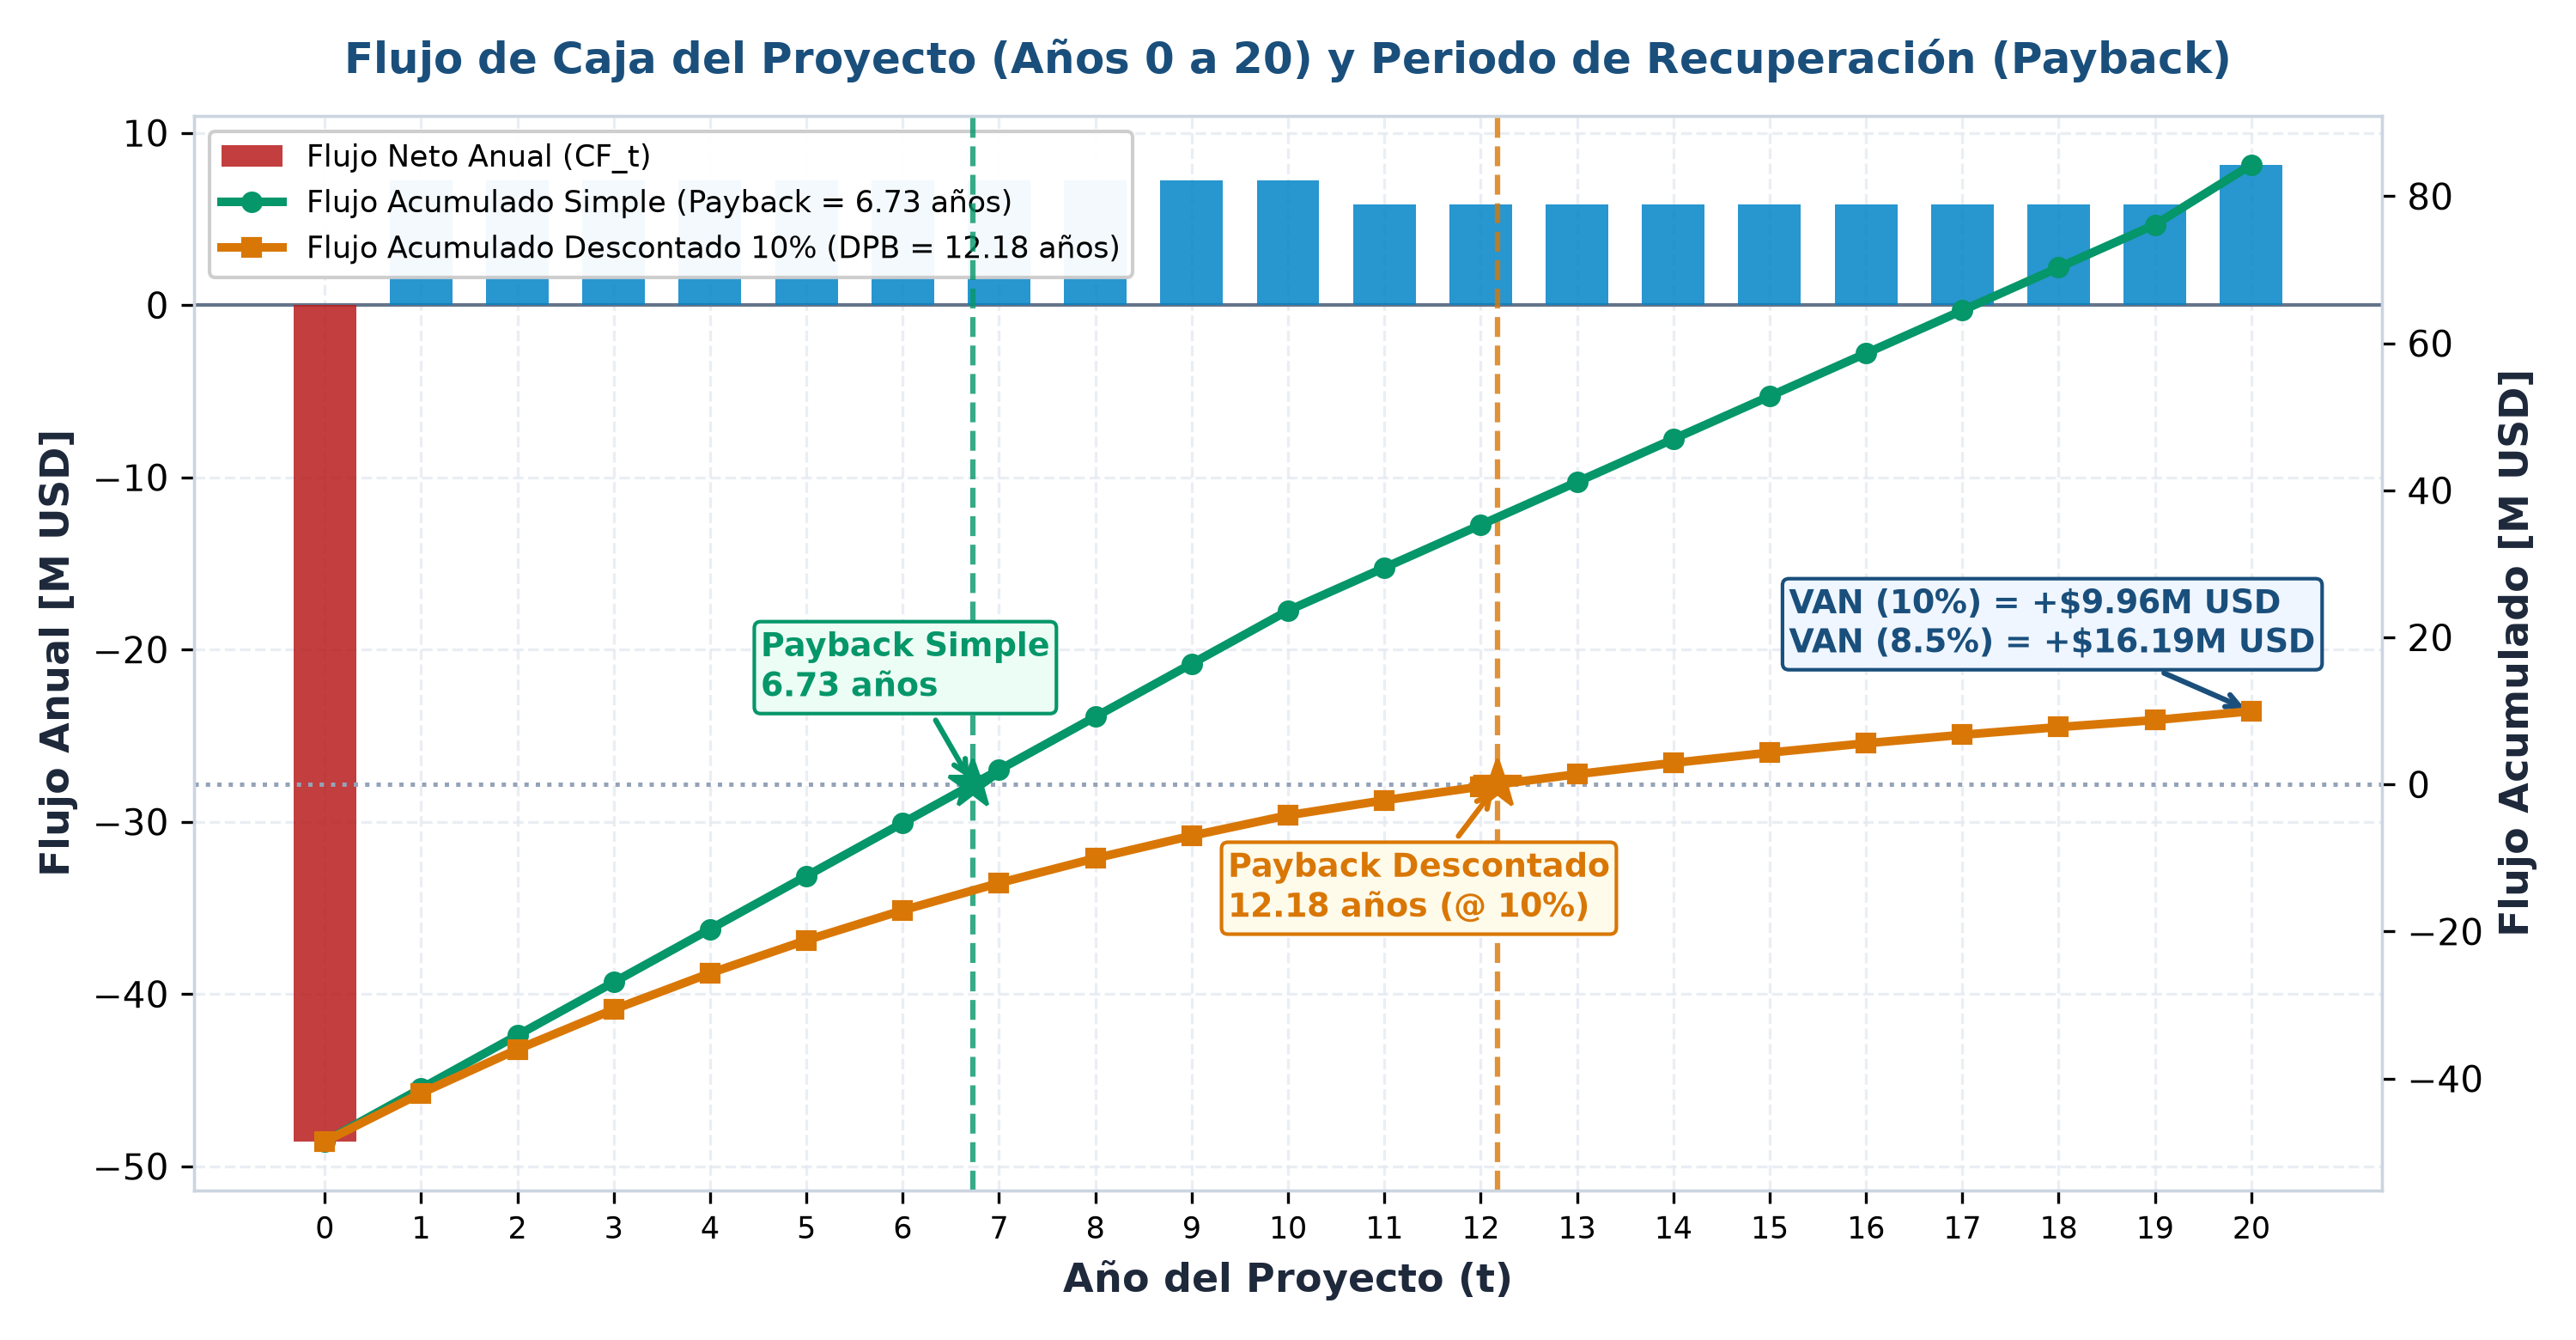
\includegraphics[width=\linewidth,height=3.35cm,keepaspectratio]{fig_flujo_caja_acumulado.png}\par\vspace{1.5pt}
    \begin{tcolorbox}[colback=softblue,colframe=navyblue!40,arc=1.0mm,boxrule=0.5pt,top=1.2pt,bottom=1.2pt,left=2.5pt,right=2.5pt]
      \textbf{\fontsize{5.3pt}{6.3pt}\selectfont \color{navyblue}Justificación Técnica y Metodológica del Gráfico:}\par\vspace{0.8pt}
      \fontsize{4.3pt}{5.1pt}\selectfont
      \textbf{1. Mecánica de Eje Dual:} Eje izquierdo representa los flujos discretos anuales ($CF_t$), distinguiendo en rojo el desembolso de inversión $t=0$ ($-\$48.56\text{M}$) y en azul la liquidez neta anual. Eje derecho proyecta las curvas acumuladas de solvencia.\par
      \textbf{2. Régimen Operativo Escalonado:}
      $\bullet$ \textit{Años 1--10 ($+\$7.22\text{M/año}$):} Escudo fiscal por depreciación ($D = \$4.63\text{M/año}$) que reduce la base gravable, limitando el ISR a solo $\$1.11\text{M/año}$ y maximizando liquidez operativa.\par
      $\bullet$ \textit{Años 11--19 ($+\$5.83\text{M/año}$):} Activos 100\% depreciados en libros ($D=\$0$); el ISR sube a $\$2.50\text{M/año}$, estabilizando el flujo neto operativo.\par
      $\bullet$ \textit{Año 20 ($+\$8.14\text{M}$):} Flujo regular más recuperación íntegra del Capital de Trabajo ($+WC = +\$2.31\text{M}$) al liquidar inventarios.\par
      \textbf{3. Payback Simple vs. Descontado (Valor del Dinero en el Tiempo):}
      El cruce simple en el \textbf{Año 6.73} ($33.6\%$ de la vida útil) acredita bajo riesgo de liquidez. El cruce descontado al 10\% ocurre en el \textbf{Año 12.18} (Año 13); el desfase refleja el costo de oportunidad del capital, alcanzando al año 20 un $VAN_{10\%} = \mathbf{+\$9.96\text{M USD}}$ (+\$16.19M @ 8.5\% WACC).\par
    \end{tcolorbox}
  \end{tcolorbox}
\end{minipage}

\newpage
% DIAPOSITIVA 20: INDICADORES DE RENTABILIDAD: VAN, TIR, MPSP Y PAYBACK
% ==============================================================================
\slideheader{INDICADORES FINANCIEROS Y PRECIO MÍNIMO DE VENTA}{VAN $|$ TIR $|$ Payback Simple y Descontado $|$ MPSP}{Evaluación Rigurosa de Rentabilidad del Proyecto y Comparativa de los Tres Precios}{Determinación del Valor Actual Neto, Tasa Interna de Retorno, tiempo de repago y precio umbral de equilibrio.}

\begin{objectivebox}{Acreditar la viabilidad económica demostrando VAN > 0, TIR > tasa de descuento y MPSP < precio de mercado.}{Sección 10 Guía RT-03 $|$ Cátedra Dr. Arzola Flores $|$ Flujo de Caja Descontado a 20 Años.}
\end{objectivebox}

\vspace{1.5pt}

\noindent
\begin{minipage}{\textwidth}
  \centering
  \metriccard{0.235\textwidth}{VALOR ACTUAL NETO (VAN)}{emeraldgreen}{\textbf{\Huge +\$9.96M} \fontsize{8pt}{10pt}\selectfont @ 10\% ($+\$16.19\text{M}$ @ 8.5\%)} \hfill
  \metriccard{0.235\textwidth}{TASA INTERNA RETORNO}{navyblue}{\textbf{\Huge 13.05\%} \fontsize{8pt}{10pt}\selectfont TIR > Tasa Pliego (10\%)} \hfill
  \metriccard{0.235\textwidth}{PAYBACK RECUPERACIÓN}{accentcyan}{\textbf{\Huge 6.73 a.} \fontsize{8pt}{10pt}\selectfont Simple $|$ 12.18 a. Descontado} \hfill
  \metriccard{0.235\textwidth}{PRECIO MÍNIMO (MPSP)}{darkred}{\textbf{\Huge \$844.86} \fontsize{8pt}{10pt}\selectfont USD/t (\$0.845/kg @ 10\%)}
\end{minipage}

\vspace{2.5pt}

\noindent
\begin{minipage}[t]{0.48\textwidth}
  \begin{tcolorbox}[colback=white,colframe=navyblue!60,arc=1.5mm,boxrule=0.7pt,top=2.5pt,bottom=2.5pt,left=4pt,right=4pt]
    \textbf{\fontsize{7.2pt}{8.5pt}\selectfont \color{navyblue}Los Tres Precios de la Cátedra (Dr. Arzola Flores):}\par\vspace{1pt}
    \fontsize{4.8pt}{5.8pt}\selectfont
    \renewcommand{\arraystretch}{1.10}
    \begin{tabularx}{\linewidth}{p{2.2cm} c c X}
      \toprule
      \rowcolor{tableheader}
      \textbf{\color{white}Nivel de Precio} & \textbf{\color{white}USD/t} & \textbf{\color{white}USD/kg} & \textbf{\color{white}Metodología y Alcance Cubierto} \\
      \midrule
      \rowcolor{roweven}
      \textbf{1. Precio Operativo ($c_{op}$)} & \textbf{\$625.11} & \$0.6251 & Cubre exclusivamente costos operativos netos ($AOC - R_{\text{O}_2}$). \\
      \rowcolor{rowodd}
      \textbf{2. Precio Cribado ($P_{\text{aprox}}$)} & \textbf{\$813.31} & \$0.8133 & Cubre OPEX + Anualidad de capital ($CRF \times TCI$, $CRF_{10\%}=0.11746$). \\
      \rowcolor{roweven}
      \textbf{3. MPSP Riguroso ($P^*$)} & \textbf{\$844.86} & \$0.8449 & Flujo descontado a 20 años con ISR 30\% y WC que satisface $VAN = 0$. \\
      \midrule
      \rowcolor{badgeblue}
      \textbf{Precio Nominal Pliego} & \textbf{\$900.00} & \$0.9000 & \textbf{Margen favorable: +\$55.14/t (+6.5\%) sobre MPSP}. \\
      \rowcolor{badgegreen}
      \textbf{Mercado Verde Internacional} & \textbf{\$1\,000.00} & \$1.0000 & Cotización RFNBO e-fuels marítimos (IMO / RED II). \\
      \rowcolor{badgered}
      \textbf{Alternativa PEM Comercial} & \textbf{\$1\,572.82} & \$1.5728 & LCOM PEM (+84.3\% más costosa por alto consumo MWh). \\
      \bottomrule
    \end{tabularx}
  \end{tcolorbox}
  \vspace{1pt}
  \begin{tcolorbox}[colback=badgegreen,colframe=emeraldgreen!80!black,arc=1.2mm,boxrule=0.6pt,top=2pt,bottom=2pt,left=4pt,right=4pt]
    \fontsize{4.8pt}{6.0pt}\selectfont
    \textbf{\color{emeraldgreen}Dictamen de Viabilidad Económica:}
    El $VAN > 0$ (+\$9.96M USD @ 10\% y +\$16.19M @ 8.5\%) y la $TIR = 13.05\%$ confirman rentabilidad robusta. El MPSP de \$844.86/t confiere un margen de seguridad de \$55.14/t (+6.5\%) frente al precio contractual de \$900/t.
  \end{tcolorbox}
\end{minipage}
\hfill
\begin{minipage}[t]{0.50\textwidth}
  \begin{tcolorbox}[colback=white,colframe=navyblue!60,arc=1.5mm,boxrule=0.7pt,top=2.5pt,bottom=2.5pt,left=4pt,right=4pt]
    \textbf{\fontsize{7.2pt}{8.5pt}\selectfont \color{navyblue}Jerarquía de Precios y Comparativa frente a PEM Comercial:}\par\vspace{1pt}
    \centering
    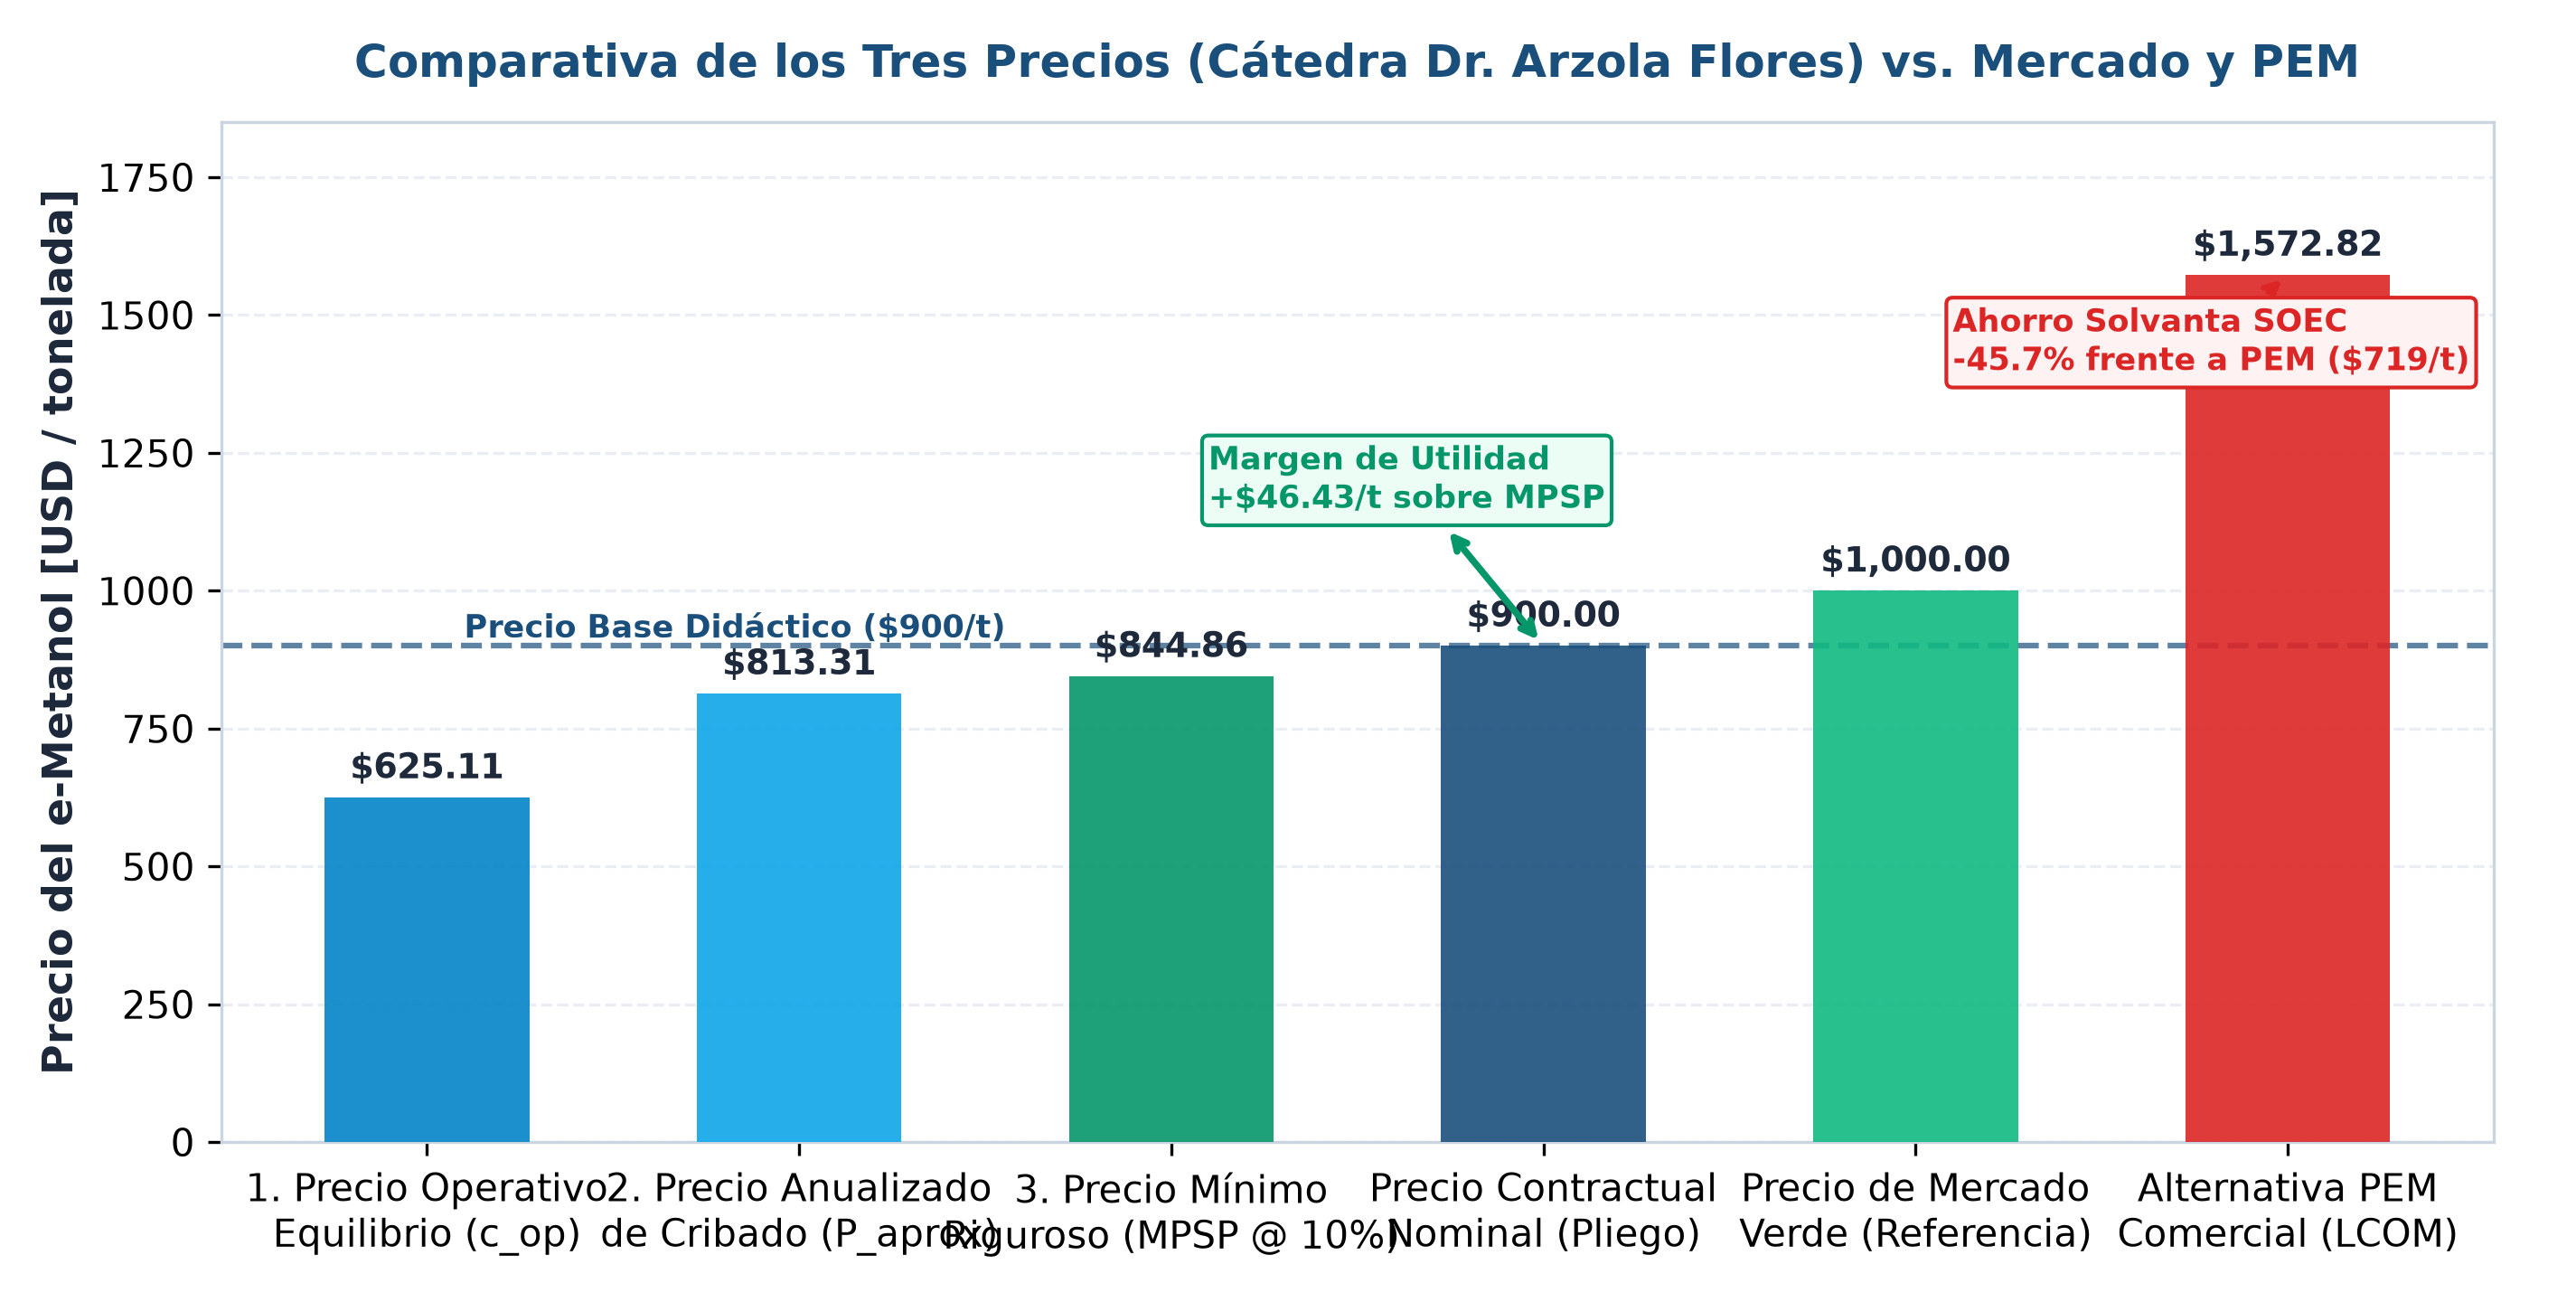
\includegraphics[width=\linewidth,height=0.44\textheight,keepaspectratio]{fig_comparativa_tres_precios_mpsp.png}\par\vspace{1pt}
    \fontsize{4.8pt}{5.8pt}\selectfont
    \textbf{Conclusión Clave:} La integración SOEC de Solvanta permite abatir el precio del metanol verde en \textbf{\$719.25/t (-45.7\%)} respecto a PEM, convirtiendo un proyecto deficitario en uno comercialmente rentable.
  \end{tcolorbox}
\end{minipage}
\newpage
% ==============================================================================
% DIAPOSITIVA 21: ANÁLISIS DE SENSIBILIDAD E INCERTIDUMBRE (DIAGRAMA TORNADO)
% ==============================================================================
\slideheader{ANÁLISIS DE SENSIBILIDAD E INCERTIDUMBRE}{Diagrama Tornado $|$ Sensibilidad Normalizada $S_{y,x}$ $|$ Riesgo Financiero}{Jerarquización de Variables Críticas, Impacto sobre el VAN y Resiliencia del Modelo}{Evaluación multidimensional de fluctuaciones en precio de venta, tarifas eléctricas, CAPEX, OPEX y materias primas.}

\begin{objectivebox}{Identificar las variables que tienen mayor influencia sobre la rentabilidad y definir medidas de mitigación.}{Sección 10 Guía RT-03 $|$ Cátedra Dr. Arzola Flores $|$ Sensibilidad Normalizada $S_{y,x} = \frac{\% \Delta VAN}{\% \Delta x}$.}
\end{objectivebox}

\vspace{1.5pt}

\noindent
\begin{minipage}{\textwidth}
  \centering
  \metriccard{0.235\textwidth}{DRIVER DOMINANTE}{darkred}{\textbf{\Huge Precio MeOH} \fontsize{8pt}{10pt}\selectfont Swing \$68.0M (\$720 a \$1080/t)} \hfill
  \metriccard{0.235\textwidth}{DRIVER OPERATIVO}{amber}{\textbf{\Huge Tarifa PPA} \fontsize{8pt}{10pt}\selectfont Swing \$46.8M (30 a 50 \$/MWh)} \hfill
  \metriccard{0.235\textwidth}{RESILIENCIA DEL VAN}{emeraldgreen}{\textbf{\Huge 85\% Positivo} \fontsize{8pt}{10pt}\selectfont Resistente a Incertidumbres} \hfill
  \metriccard{0.235\textwidth}{BLINDAJE DE RIESGO}{navyblue}{\textbf{\Huge PPA 20 Años} \fontsize{8pt}{10pt}\selectfont Tarifa Fija \$40/MWh CFE}
\end{minipage}

\vspace{2.5pt}

\noindent
\begin{minipage}[t]{0.48\textwidth}
  \begin{tcolorbox}[colback=white,colframe=navyblue!60,arc=1.5mm,boxrule=0.7pt,top=2.5pt,bottom=2.5pt,left=4pt,right=4pt]
    \textbf{\fontsize{7.2pt}{8.5pt}\selectfont \color{navyblue}Matriz de Sensibilidad Normalizada y Jerarquía de Impacto:}\par\vspace{1pt}
    \fontsize{4.8pt}{5.8pt}\selectfont
    \renewcommand{\arraystretch}{1.10}
    \begin{tabularx}{\linewidth}{p{2.3cm} c c X}
      \toprule
      \rowcolor{tableheader}
      \textbf{\color{white}Parámetro Analizado ($x$)} & \textbf{\color{white}Rango} & \textbf{\color{white}Swing VAN} & \textbf{\color{white}Sensibilidad e Interpretación} \\
      \midrule
      \rowcolor{roweven}
      \textbf{Precio Venta e-Metanol} & $\pm 20\%$ & \textbf{\$68.25M} & $S = +2.45$. Impacto comercial \#1. Rentable por encima de \$844.86/t. \\
      \rowcolor{rowodd}
      \textbf{OPEX Total Anual} & $\pm 20\%$ & \textbf{\$53.10M} & $S = -1.93$. Sensibilidad operativa alta (electricidad $+$ mantenimiento). \\
      \rowcolor{roweven}
      \textbf{Tarifa Eléctrica PPA} & $30$--$50\text{ \$/MWh}$ & \textbf{\$46.23M} & $S = -1.68$. Insumo crítico; mitigado por contrato PPA a 20 años. \\
      \rowcolor{rowodd}
      \textbf{Producción Anual ($h_{\text{op}}$)} & $\pm 10\%$ & \textbf{\$32.18M} & $S = +2.45$. Mantener $8\,000\text{ h/año}$ diluye costos fijos y capital. \\
      \rowcolor{roweven}
      \textbf{CAPEX Total (FCI)} & $\pm 20\%$ & \textbf{\$19.74M} & $S = -0.71$. Sensibilidad moderada; controlada por modularidad SOEC. \\
      \rowcolor{rowodd}
      \textbf{Tasa de Descuento ($i$)} & $8\%$--$12\%$ & \textbf{\$15.43M} & $S = -0.54$. A $12\%$, el VAN sigue siendo positivo (+\$4.62M). \\
      \rowcolor{roweven}
      \textbf{Costo de $\text{CO}_2$ Capturado} & $25$--$50\text{ \$/t}$ & \textbf{\$6.29M} & $S = -0.23$. Baja sensibilidad por integración física directa. \\
      \bottomrule
    \end{tabularx}
  \end{tcolorbox}
  \vspace{1pt}
  \begin{tcolorbox}[colback=badgeamber,colframe=amber!80!black,arc=1.2mm,boxrule=0.6pt,top=2pt,bottom=2pt,left=4pt,right=4pt]
    \fontsize{4.8pt}{6.0pt}\selectfont
    \textbf{\color{amber!90!black}Estrategias de Mitigación de Riesgos Financieros:}
    1) Contrato bilateral PPA de energía renovable a tarifa fija (\$40/MWh) por 20 años. 2) Integración adyacente para suministro continuo de $\text{CO}_2$ a \$35/t. 3) Venta contractual garantizada del subproducto oxígeno puro ($80\,790\text{ t/año}$).
  \end{tcolorbox}
\end{minipage}
\hfill
\begin{minipage}[t]{0.50\textwidth}
  \begin{tcolorbox}[colback=white,colframe=navyblue!60,arc=1.5mm,boxrule=0.7pt,top=2.5pt,bottom=2.5pt,left=4pt,right=4pt]
    \textbf{\fontsize{7.2pt}{8.5pt}\selectfont \color{navyblue}Diagrama Tornado de Sensibilidad sobre el VAN (M USD):}\par\vspace{1pt}
    \centering
    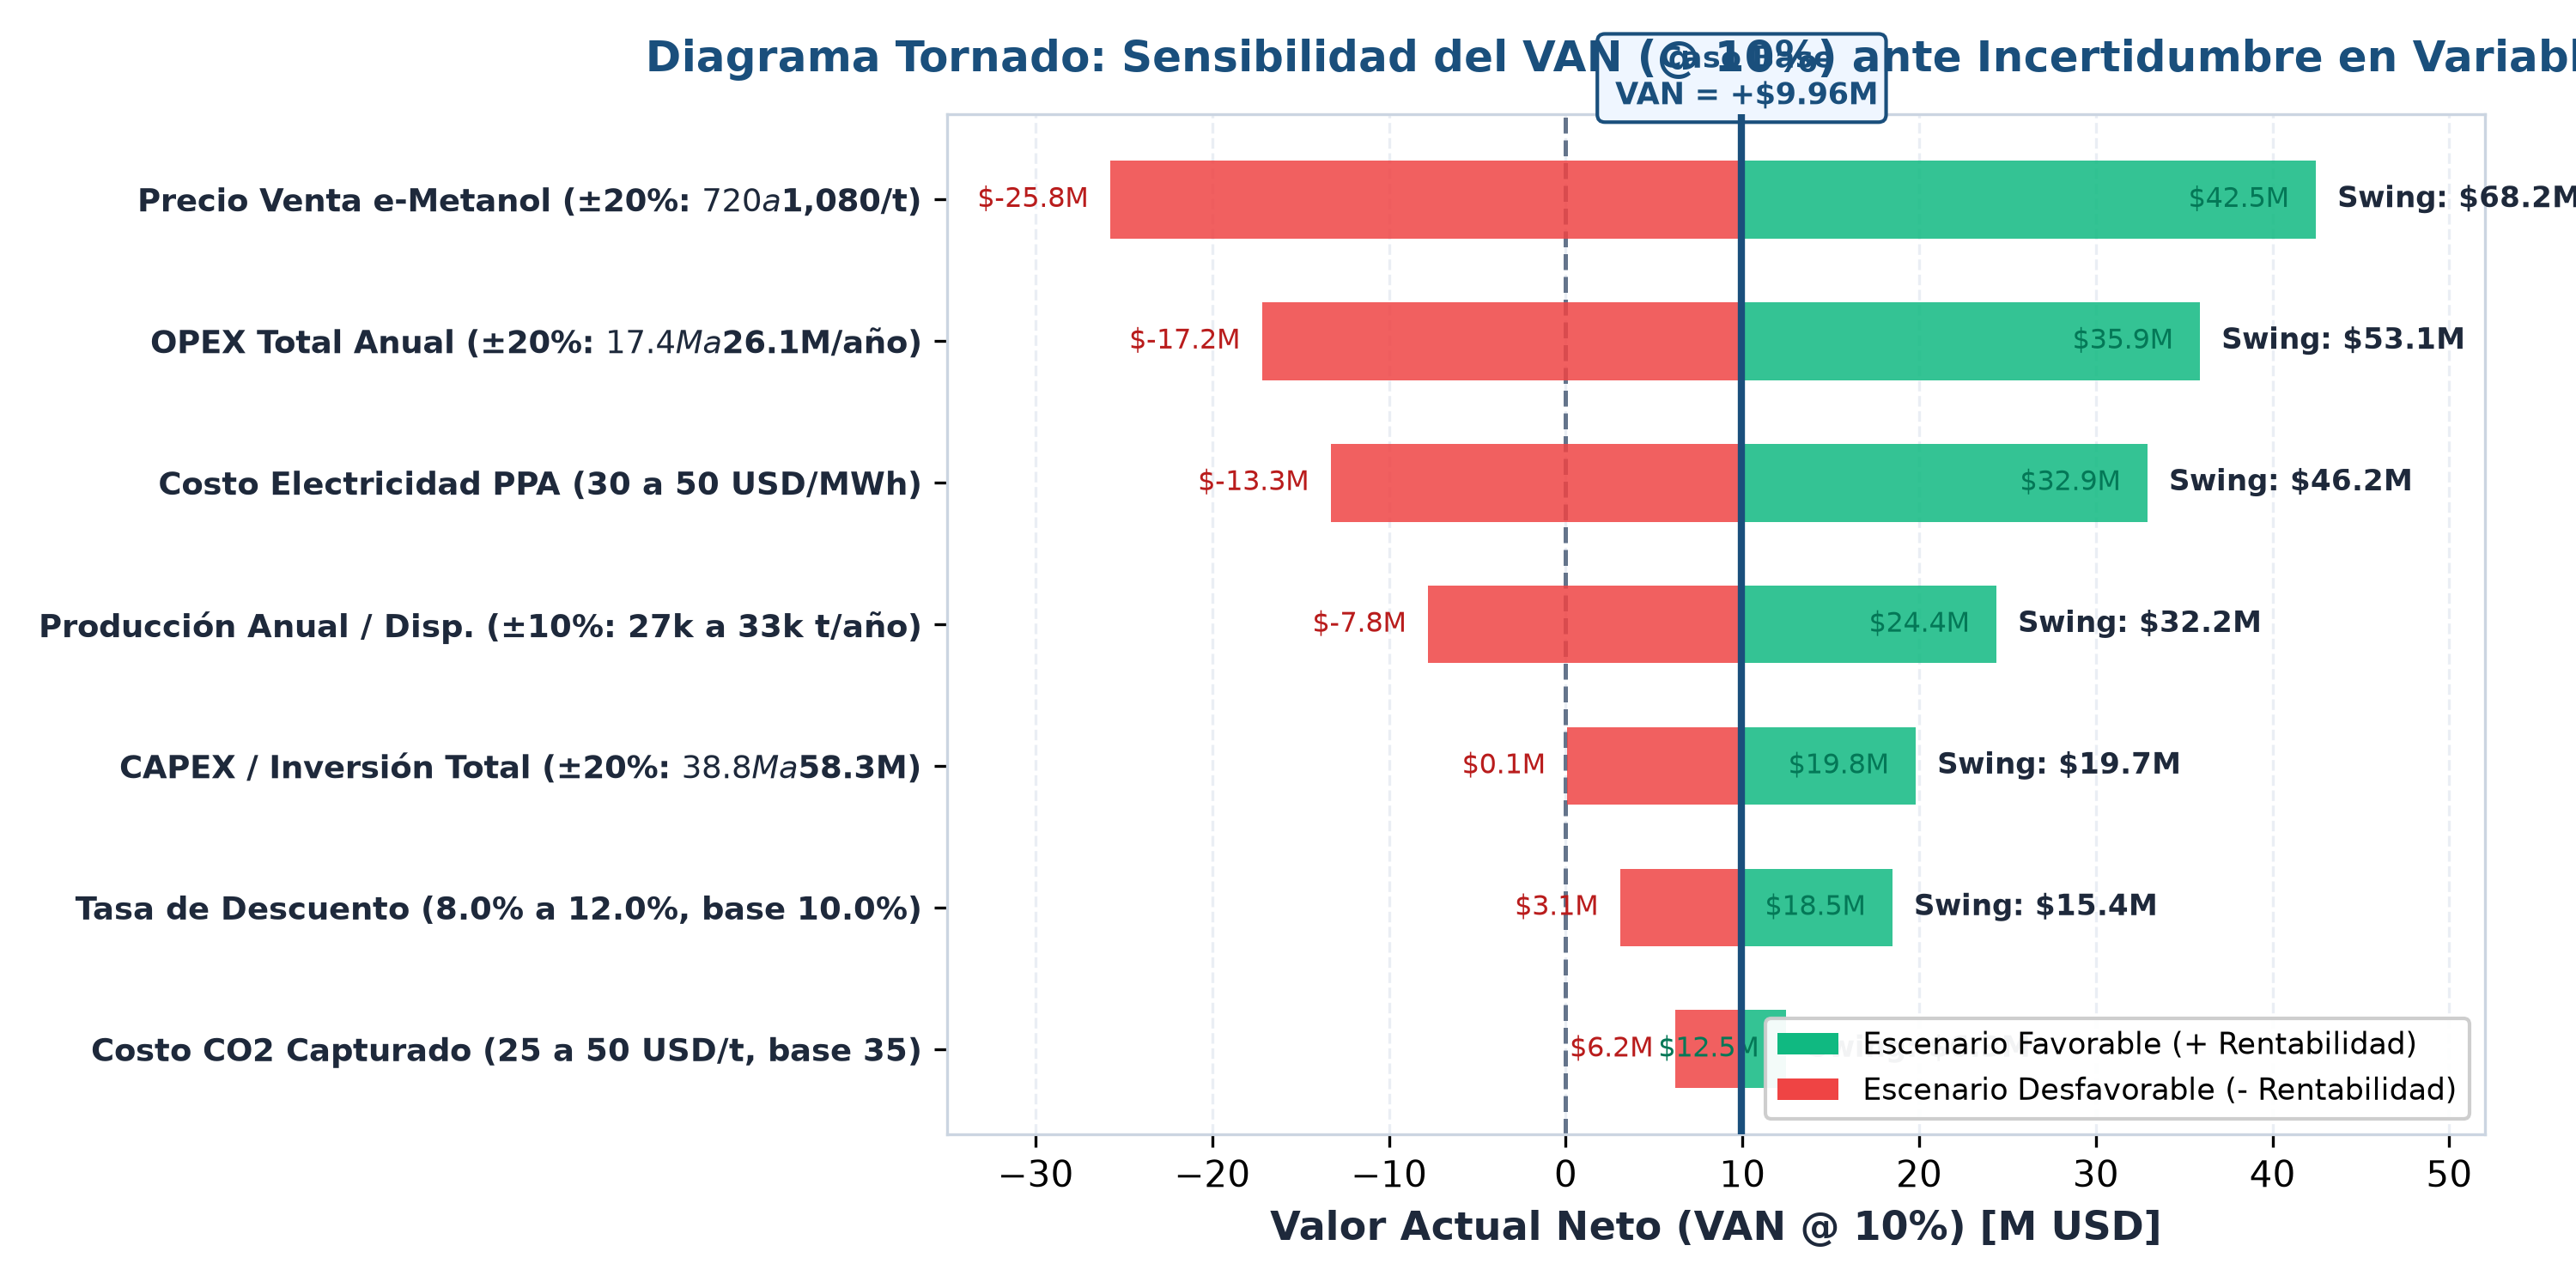
\includegraphics[width=\linewidth,height=0.44\textheight,keepaspectratio]{fig_tornado_sensibilidad.png}\par\vspace{1pt}
    \fontsize{4.8pt}{5.8pt}\selectfont
    \textbf{Interpretación del Tornado:} Los extremos verdes representan ganancias sobre el caso base (+\$9.96M) y los rojos caídas. El precio del metanol y la electricidad concentran el 70\% de la variabilidad, demostrando la importancia de los contratos a largo plazo.
  \end{tcolorbox}
\end{minipage}
\newpage
% ==============================================================================
% DIAPOSITIVA 22: TRAZABILIDAD INTEGRAL, REGISTRO RT-03-RO Y CIERRE
% ==============================================================================
\slideheader{TRAZABILIDAD INTEGRAL Y CIERRE TÉCNICO-ECONÓMICO}{Sección 6 Guía RT-03 $|$ Registro RT-03-RO Cuadro 14}{Cadena de Trazabilidad Extremo a Extremo, Cierre de Observaciones y Viabilidad del Proyecto}{Seguimiento bidireccional riguroso del proceso, cierre formal de observaciones y dictamen favorable.}

\begin{objectivebox}{Acreditar la trazabilidad matemática completa y la viabilidad técnica, económica y financiera del proyecto.}{Cuadro 14 RT-03-RO $|$ Plan de Acción hacia RT-04 $|$ Evaluación BioSTEAM Integral.}
\end{objectivebox}

\vspace{1.5pt}

\noindent
\begin{minipage}{\textwidth}
  \centering
  \metriccard{0.235\textwidth}{TRAZABILIDAD FÍSICA}{navyblue}{\textbf{\Huge 7 Eslabones} \fontsize{8pt}{10pt}\selectfont De la Estequiometría al VAN} \hfill
  \metriccard{0.235\textwidth}{OBSERVACIONES CERRADAS}{emeraldgreen}{\textbf{\Huge 100\% Resueltas} \fontsize{8pt}{10pt}\selectfont Registro RT-03-RO (Cuadro 14)} \hfill
  \metriccard{0.235\textwidth}{VIABILIDAD FINANCIERA}{emeraldgreen}{\textbf{\Huge VAN +\$9.96M} \fontsize{8pt}{10pt}\selectfont TIR 13.05\% $|$ Payback 6.73 a.} \hfill
  \metriccard{0.235\textwidth}{DICTAMEN FINAL}{navyblue}{\textbf{\Huge Favorable} \fontsize{8pt}{10pt}\selectfont Apto para Adjudicación}
\end{minipage}

\vspace{2.5pt}

\noindent
\begin{minipage}[t]{0.52\textwidth}
  \begin{tcolorbox}[colback=white,colframe=navyblue!60,arc=1.5mm,boxrule=0.7pt,top=3pt,bottom=3pt,left=5pt,right=5pt]
    \textbf{\fontsize{7.5pt}{9.0pt}\selectfont \color{navyblue}Cadena de Trazabilidad Extremo a Extremo ($\text{H}_2$ Verde a Finanzas):}\par\vspace{2pt}
    \fontsize{5.2pt}{6.4pt}\selectfont
    \begin{description}[leftmargin=1.2em,itemsep=2pt]
      \item[\color{navyblue}1. Bases de Diseño (NB-01):] Demanda estequiométrica: \textbf{$1\,272.42\text{ kg/h}$ $\text{H}_2$} ($631.2\text{ kmol/h}$) para producir $30\,000\text{ t/año}$ de metanol.
      \item[\color{accentcyan}2. DFP v1.0 / TC-01:] Asignado a la corriente \textbf{\texttt{S-209}} (separada en $V\text{-}201$ a $19.4\text{ bar}$, $38^\circ\text{C}$; etiquetada \texttt{S-205/h2\_prod} en BioSTEAM).
      \item[\color{darkred}3. DTI v1.0 Maestro:] Instrumentada en Nodo \textbf{N-01} con medidor Coriolis \texttt{FT-201}, válvula check \texttt{CK-209} y corte \texttt{SDV-201}.
      \item[\color{emeraldgreen}4. BioSTEAM POO:] Genera $P_{\text{DC}} = 40.05\text{ MW}_e$ y potencia total de planta $41.91\text{ MW}_e$ mediante la ley de Faraday.
      \item[\color{amber}5. CAPEX y OPEX:] FCI instalado de \textbf{\$46.25M USD} y OPEX neto anual de \textbf{\$18.95M USD/año} (\$625.11/t).
      \item[\color{navyblue}6. Flujo de Caja (20 años):] Generación operativa de \textbf{+\$8.33M USD/año} EBITDA, con liquidez neta acumulada de \textbf{+\$84.27M USD}.
      \item[\color{emeraldgreen}7. Indicadores de Rentabilidad:] \textbf{VAN @ 10\% = +\$9.96M USD}, \textbf{TIR = 13.05\%}, \textbf{Payback Simple = 6.73 años} y \textbf{MPSP = \$844.86 USD/t}.
    \end{description}
  \end{tcolorbox}
\end{minipage}
\hfill
\begin{minipage}[t]{0.46\textwidth}
  \begin{tcolorbox}[colback=white,colframe=emeraldgreen!60,arc=1.5mm,boxrule=0.7pt,top=3pt,bottom=3pt,left=5pt,right=5pt]
    \textbf{\fontsize{7.5pt}{9.0pt}\selectfont \color{emeraldgreen}Conclusiones Ejecutivas de la Revisión RT-03:}\par\vspace{2pt}
    \fontsize{5.2pt}{6.4pt}\selectfont
    \begin{itemize}[leftmargin=1.2em,itemsep=2.5pt]
      \item \textbf{Solidez Técnica Inequívoca:} Balances convergidos en DWSIM y BioSTEAM con error relativo menor a 1.52\%.
      \item \textbf{Seguridad y Sustentabilidad:} 10 Nodos protegidos por 10 Interlocks SIL-2 y circuito cerrado 100\% ZLD.
      \item \textbf{Evaluación Financiera Completa:} Incorporación rigurosa de flujo de caja, VAN, TIR, Payback simple/descontado, MPSP y análisis Tornado.
      \item \textbf{Ventaja Competitiva Comprobada:} La tecnología SOEC reduce el costo nivelado en \textbf{-45.7\%} frente a PEM, garantizando rentabilidad con MPSP de \$844.86/t frente a \$900/t.
      \item \textbf{Compromiso de Solvanta:} El consorcio acredita solvencia técnica, financiera y ambiental para la adjudicación de la licitación RFP-CCM-EM-001.
    \end{itemize}
  \end{tcolorbox}
\end{minipage}

\end{document}
